\documentclass[12 pt,a4 paper ]{scrreprt}
 
\usepackage[utf8]{inputenc}
\usepackage[naustrian]{babel}
\usepackage{lmodern}
\usepackage[T1]{fontenc}
\usepackage{graphicx}
\usepackage{amsmath}
\usepackage{float}
\usepackage{amsmath,amssymb,amstext}
%\usepackage{pgfplots}

\usepackage[headsepline,plainheadsepline]{scrpage2}
\pagestyle{scrheadings}
\ihead[\rightmark]{\rightmark} \chead[]{}
%\ohead[\pagemark]{\pagemark} \cfoot[]{}

\automark{chapter}
\renewcommand{\chaptermark}[1]{\markright{\ #1}}










\begin{document}
\tableofcontents
\chapter{Einführung}
\section{Einleitung, Ziele und Vorgehensweise}
 

Die vorliegende Arbeit entstand im Rahmen meiner Diplomarbeit am Institut für Tragwerkplanung und Ingenieurholzbau.Die Diplomarbeit schließt an die vorgehenden Arbeiten von Herrn Dipl.Ing Kirchmayer und Herrn Dipl.Ing Schernberger an. Im Rahmen des Projektes " Weitgespannte Flachdeckensysteme in Holzspanbeton – Verbundweise" sind ihre Arbeiten entstanden. Sie haben in Ihren Ausarbeitungen die Grundlagen des behandelten Aufbaus erarbeitet. Die Arbeit von Herrn Schernberger befasst sich mit der allgemeinen Anwendung und den Einsatzgebieten des Holzbetons. Herr Kirchmayer hat sich in seiner Ausarbeitung mit den verschiedenen Verbundmöglichkeiten beschäftigt. Anhand der Versuchsreihen von Herrn Kirchmayer wurden verschiedene Verbindungsmöglichkeiten untersucht. Durch diese Arbeit ist der dargestellte Sandwichaufbau[abb..] entstanden. Dieser Aufbau wird von uns weiter verwendet


\begin{figure}[h]
\begin{center}
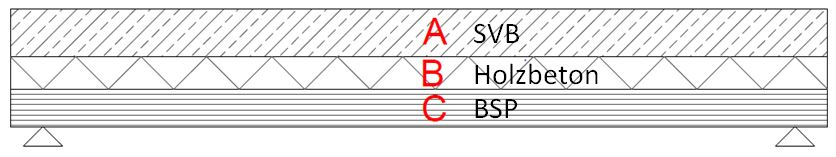
\includegraphics[scale =0.7]{sandwichaufbau.png}
\caption{Sandwichaufbau}
\end{center}
\end{figure}

Ziele und Vorgehensweise

Das erste übergeordnete Ziel dieser Arbeit ist die Entwicklung von einem Sandwichaufbau aus CLT, Holzbeton und SCC. Dabei stehen die Fragen des Verbundverhaltens bzw. der Anwendung von den verschiedenen Verbindungsmittel im Vordergrund. Das zweite Ziel dieser Arbeit ist die Nachrechnung der Versuchsergebnisse mit den „y-Verfahren“ und dem Finite Elemente Programm „Sofistik“. Es sollen die Grundlagen zur Bemessung des Sandwichaufbaus entwickelt werden. 
Zusätzlich ist eine ökonomische Betrachtung des Sandwichaufbaus zu erstellen und einen Vergleich mit den gängigen Deckensystemen zu erarbeiten.


Die genannten Ziele sollen mit Hilfe von den experimentellen Großbauteilversuchen erzielt werden. Dabei wird ausschließlich das Kurzzeitverhalten des Sandwichaufbaus untersucht. Um einen das Langzeitverhalten auch zu berücksichtigen wird die Durchbiegung mit l/400 begrenzt, bei der Belastung für einen Büroraum oder Wohnraum.



\newpage{}
Im Nachfolgenden Ablaufdiagramm ist die Vorgehensweise dieser Arbeit ersichtlich.

\begin{figure}[h]
\begin{center}
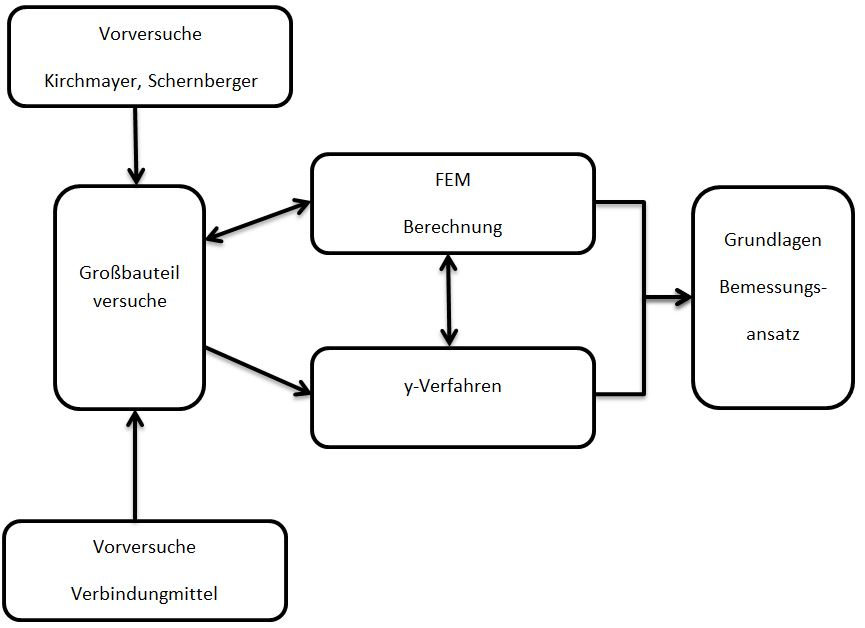
\includegraphics[scale =0.7]{ablauforganigramm.png}
\caption{Ablauforganigramm der Diplomarbeit}
\end{center}
\end{figure}




\section{Zusammenfassung der Kapitel}

\begin{enumerate}
\item Zusammenfassung von Vorarbeit 
\item Ermittlung der mechanischen Eigenschaften der Verbindungsmittel
\item Versuchaufbau und Durchführung
\item Beschreibung und Auswertung der Großbauteilversuche
\item Beschreibung der Berechnungsverfahren
\item Vergleich Berechnung Versuche und Berechnungen
\item wirtschaftliche Untersuchungen

\end{enumerate}




\chapter{Verbindungsmittel}

\section{Schrauben}

Durch den ähnlichen Aufbau des Sandwiches zum HBV-System wurden die Verbundmöglichkeiten des Systems näher untersucht und für das Sandwich adaptiert. Das am häufigsten ausgeführte HBV-System wird mit Verbundschrauben direkt vor Ort hergestellt. Vorteil dieses Systems ist die schnelle Vorbereitung da die Schrauben ohne Vorbohren in das Holz eingebohrt werden können. Es gibt mehrere Hersteller, die in der Arbeit von Herrn Dipl.Ing Schernberger [] aufgelistet sind, die dieses System anbieten. Es wird auch auf die Einsatzmöglichkeiten und die Vor- und Nachteile jedes Herstellers eingegangen. Herr Dipl.Ing Kirchmayer hat in seinen Verbundversuchen[] gezeigt, dass die Verwendung von Schrauben zu den besten Verbundverhalten des Sandwiches führen. Aufgrund dieser Erkenntnisse und der Erfordernis einer Mindestlänge der Schrauben bzw. wurde die Firma SFS kontaktiert. Die Firma besitzt Schraubenreihen mit in verschiedensten Ausführungsvarianten und entsprechenden Schraubenlängen. Um die Auswahl der Schrauben einzugrenzen, wurden folgende Eigenschaften von uns vorgegeben:


\begin{enumerate} 
	\item Einschraubwinkel: $45^\circ-50 ^\circ$
	\item Schraubenlänge: 400 mm
	\item Einschraubtechnik: ohne Vorbohren
	\item Keine Beschädigung der Schrauben beim durchbohren des Holzleichtbetons (Velox)
\end{enumerate}

Die Punkte 1 - 3 waren schon durch die Datenblätter der Firma SFS abgedeckt.
Der 4 Punkt war aufgrund der neuartigen Zusammensetzung des Sandwiches noch nicht überprüft worden. Daher wurde von uns, in Zusammenarbeit mit der Firma SFS verschiedene Schraubentypen getestet. 
\newline{}
\newline{}
Die Schrauben unterschieden sich in: 

\begin{itemize}
	\item Schraubenkopfform
	\item Gewindeanordnung
	\item Schaftform
	\item Spitze
\end{itemize}

Ausgesuchte Schraubentypen: 


\begin{itemize}
	\item WR – dxL
	\item TWIN – DU dxL Sichel
	\item WT – T dxL 
	\item TWIN – DU dxL
	\item WR – T  dxL
\end{itemize}
	
\subsection{Schraubentype:	 WR – dxL}
Das Befestigungssystem WR findet hauptsächlich Anwendung für große Querschnitte im Bereich der Verbindungen, Verstärkungen und Stahl-Holz-Anschlüsse. Die Schrauben sind aus Kohlenstoffstahl gefertigt. Der Schraubendurchmesser ist wählbar zwischen 9 mm und 13 mm. Die Schrauben sind in den Längen von  250 mm bis 1000 mm verfügbar. Die Oberfläche der Schraube ist mit einem Durocoat für den Korrosionsschutz überzogen. 

\begin{figure}[h]
\begin{center}
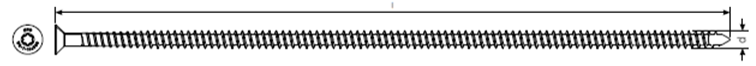
\includegraphics[scale =0.7]{WR-dxL.png}
\caption{Schraubentype: WR - dxL}
\end{center}
\end{figure}


Die Vorteile die vom Hersteller angegeben werden sind[]:

\begin{itemize}
	\item Sehr hohe Leitungsfähigkeit
	\item Breites Anwendungsspektrum
	\item Verschraubung auch paralell zur Faserrichtung möglich
	\item Keine Abminderung der Tragfähigkeit von $90^\circ  -  45^\circ$ zur Faser
	\item Verarbeitung ohne Vorbohren
	\item Geringe Spaltneigung
	\item Unsichtbare Verbindung
\end{itemize}


\subsection{Schraubentype: TWIN-UD dxL Sichel }
Das System TWIN DU wird seit Jahren für die Befestigung von Aufsparrendämmung auf Dächern  und hinterlüftete Fassaden verwendet. Die Schrauben sind aus Kohlenstoffstahl gefertigt. Der Schraubendurchmesser beträgt 7,5 mm  und die Schraubenlänge variiert im Bereich von 160 mm – 480 mm. Die Oberfläche der Schraube ist mit einem Durocoat als Korossionsschutz überzogen.

\begin{figure}[h]
\begin{center}
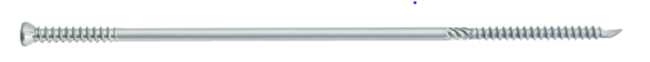
\includegraphics[scale =0.7]{TWIN-UDdxLSichel.png}
\caption{Schraubentype: TWIN-UD dxL Sichel}
\end{center}
\end{figure}


Die Vorteile die vom Hersteller angegeben werden sind[]:

\begin{itemize}
	\item Holzbohrspitze reduziert die Spaltgefahr des 	Holzes
	\item Optimiertes Doppelgewinde ohne		 Gangunterschied
	\item Rändel für erleichtertes Eindrehen
	\item Mehr Leistung durch angepasste 	Gewindedurchmesser
	\item Hohe Traglast auf Zug und Druck dank 	Doppelgewinde
	\item Minimale Wärmebrücken bei vollflächiger 	Dämmung
	\item Einfache Arbeitsschritte- minimaler 	Arbeitsaufwand
	\item Dämmstärken von 60 mm - 300 mm möglich
\end{itemize}


\subsection{Schraubentype: WT – T dxL }
Das Befestigungssystem WT ist für den universellen Einsatz im konstruktiven Holzbau in Gebrauch. Die Schrauben sind aus Kohlenstoffstahl gefertigt. Der Schraubendurchmesser ist wählbar zwischen 6,5 mm und 8,2 mm. Die Schrauben sind in den Längen von  65 mm – 330 mm verfügbar. Die Oberfläche der Schraube ist mit einem Durocoat als Korrosionsschutz überzogen.

\begin{figure}[h]
\begin{center}
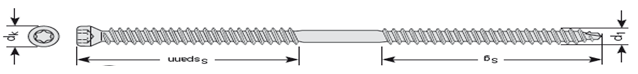
\includegraphics[scale =0.7]{WT-TdxL.png}
\caption{Schraubentype: WT-T dxL}
\end{center}
\end{figure}

Die Vorteile die vom Hersteller angegeben werden sind[]:

\begin{itemize}
	\item Einfache und sichere Berechnung
	\item Vielfältiges Anwendungsspektrum
	\item Dauerhafte Verbindung  bei hoher Tragfähigkeit
	\item Schnelles, effizientes Verarbeiten ohne Vorbohren
	\item Formschlüssige Verbindung  dank Doppelgewinde
	\item Hoher Brandwiderstand
	\item Anspruchsvolle Ästhetik dank versenkter Befestigungsmittel
	
\end{itemize}

\subsection{Schraubentype:	 WR – T  dxL}
Das Befestigungssystem WR-T ist für den universellen Einsatz im konstruktiven Holzbau in Gebrauch. Die Schrauben sind aus Kohlenstoffstahl gefertigt. Der Schraubendurchmesser ist wählbar zwischen 9 mm und 13 mm. Die Schrauben sind in den Längen von  250 mm – 1000 mm verfügbar. 

\begin{figure}[h]
\begin{center}
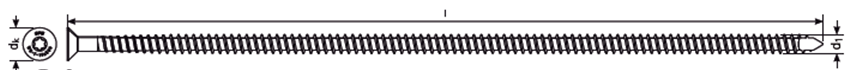
\includegraphics[scale =0.7]{WR-TdxL.png}
\caption{Schraubentype: WT-T dxL}
\end{center}
\end{figure}

Die Vorteile die vom Hersteller angegeben werden sind[]:

\begin{itemize}
	\item Hohe Tragfähigkeit
	\item Einfache Verarbeitung
	\item Hoher Brandwiderstand der Verbindung
	\item Schnelle Montage ohne Vorbohen
	\item Verbindungsmittel nicht sichtbar
\end{itemize}

\subsection{Versuchsaufbau für Schrauben}

Um Beschädigung beim Durchbohren zu sehen, wurde ein Aufbau gewählt, der der tatsächlichen Verwendung bei den Großbauteilversuchen entspricht. Es wurden 4 Lagen Veloxplatten zu je 5cm übereinandergelegt und mit Klemmzangen zusammengehalten. Um das Durchbohren und die anschließende Besichtigung der Schrauben zu ermöglichen, wurden die Platten auf Holzböcken gelagert.  

\begin{figure}
\begin{center}
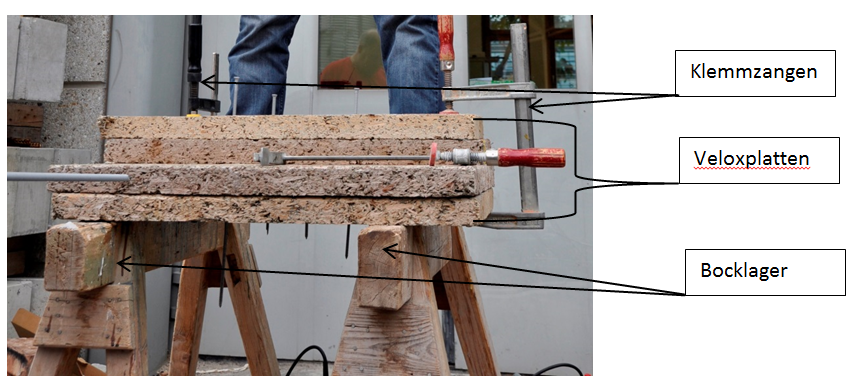
\includegraphics[scale =0.7]{Schraubenversuchsaufbau.png}
\caption{ Schraubenversuchsaufbau}
\end{center}
\end{figure}

\subsection{Versuchsauswertung}

In der Abbildung \ref{Schraubenauswertung} sind die Schraubenspitzen nach dem Durchbohren der Veloxplatten dargestellt. ES ist ersichtlich, dass keine der Schrauben beschädigt worden ist. Dies ist auf das poröse Material zurückzuführen, dass keine mineralischen Bestandteile besitzt. Weiters war beim Einbohren der Schrauben, kein Unterschied im Kraftaufwand festzustellen. 

\begin{figure}[h!]
\begin{center}
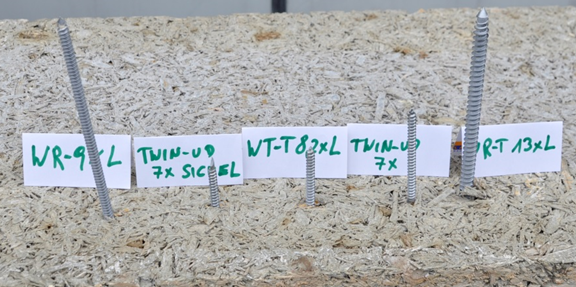
\includegraphics[scale =0.8]{Schraubenauswertung.png}
\caption{ Schraubenwertung}
\label{Schraubenauswertung}
\end{center}
\end{figure}



Die Auswahl der Schraube erfolgte Aufgrund der nachstehend Kriterien.
Um über den gesamten Einbohrvorgang eine Führung zu gewährleisten, wurde eine Gewindeanordnung über die gesamte Schraubenlänge bevorzugt. Zusätzlich kann durch das Gewinde, ein besserer Auszugswiederstand aus dem Beton gewährleistet werden. 
Die Spitze war ein weiteres Entscheidungskriterium, hierbei wurde darauf geachtet, dass sich die Schraube problemlos mit einem einfachen Hilfsmittel (Hammer) ansetzen ist. 
Der Schraubenkopf sollte eine große Fläche vorweisen, damit ein guter  Verbund mit dem Beton entsteht. 
?? Durch die Vorgabe, von einer lichten Weite bis zu 10 m und damit die einhergehende Bauteilerhöhung muss auch die Schraubenlänge noch erweiterbar sein.??
\newline{}

Alle Kriterien erfüllte die Schraubentype: \textbf{WR – T dxL} 




\section{Kleber}
Unter Kleben (nach EN DIN 923,[]) versteht man: Fügen gleicher oder ungleicher Werkstoffe unter Verwendung eines Klebstoffes. 

Klebstoffe sind (nach EN DIN 923,[]) nichtmetallische Stoffe, die Fügeteile durch Flächenhaftung und innere Festigkeit(Adhäsion und Kohäsion) verbinden.


\subsection{Einteilung}

Die Einteilung der Klebestoffe wird im Buch Kleben von Gerd Habenicht[] auf zwei Arten angeführt. Zum einem auf der chemischen Basis und nach dem Abbindemechanismus. 
\begin{figure}[h]
\begin{center}
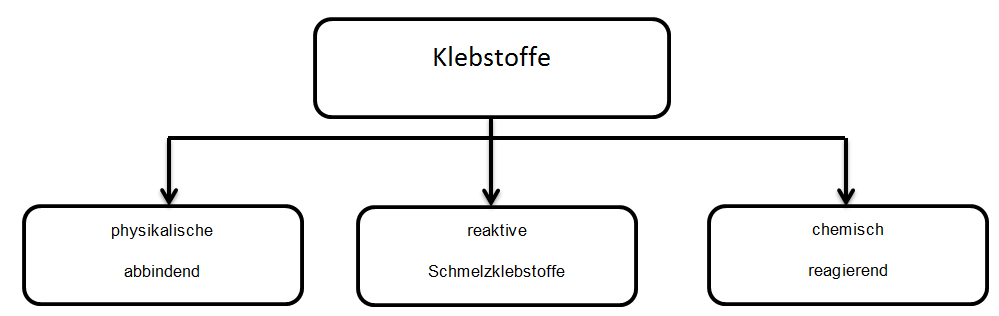
\includegraphics[scale =0.6]{einteilungderklebstoffe.png}
\caption{ Einteilung der Klebstoffe nach dem Abbindemechanismus, []}
\label{Einteilung der Kelbstoffe}
\end{center}
\end{figure}


\subsection{Vor- und Nachteile der Klebverbindungen}

Im Fachbuch für Kleben[4], hat Habenich die Vor- und Nachteile des Klebens gegenüber: Schweißen, Löten, Schrauben, und Nieten beschrieben. 
\newline{}

\textbf{Vorteile von Klebungen,[4, Tabelle 7.1]}
\begin{itemize}
	\item Gleichmäßige Spannungsverteilung senkrecht zur Belastungsrichtung 
	\item Keine Thermische Gefügebeeinflussung
	\item Kein thermisch bedingter Bauteilverzug
	\item Verbindungsmöglichkeit für unterschiedliche Materialkomponenten
	\item Gewichtsersparnis, Leichtbau
	\item Verbingungsmöglichkeit für sehr wärmeempfindliche Werkstoffe
	\item Festigkeitserhöhung in Verbindung mit Schrauben
	\item Hohe dynamische Festigkeit, hohe Schwingunsdämpfung
	\item Möglichkeit zur Automatisierung
\end{itemize}


\textbf{Nachteile von Klebungen, [4, Tabelle 7.2]}

\begin{itemize}
	\item Einfluss der Zeit auf den Verfahrensablauf
	\item Oberflächenvorbehandlung der Fügeteile
	\item Begrenzte thermische Frombeständigkeit
	\item Sorgfältige Prozesskontrolle
	\item Alterungsabhängigkeit der Klebschicht und Grenzschicht
	\item Aufwendige Kontrollverfahren
	\item Geringe Schälwiederstände, Kriechneigung
	\item Begrenzte Reparaturmöglichkeiten
	\item Aufwendige Festigkeitsberechnungen
	\item Demontage von Klebungen
	\end{itemize}

Bei der Auflistung der Vor -und Nachteile können die Nachteile durch die vorgesehene Verwendung fast alle entschärft werden. Die Vorteile der Verbindungsmethode sind zumeist zutreffend. Aus diesen Überlegungen ist die Anwendung der Klebeverbindung beim Sandwichbauteil gerechtfertigt.
Bei der Auswahl der verwendeten Kleber haben wir die Firma Sika hinzugezogen, da die Firma über ein großes Expertenwissen verfügt. 


\subsection{Ermitllung des Kleberbedarfs mit der Sandfleckmethode}

Um den Kleberverbrauch für poröse Bauteile zu ermitteln, wird die Sandfleckmethode angewendet.
Mit der Sandfleckmethode wird die Rauigkeit von porösen Materialien bestimmt  
und daraus kann mit einer Formelwerk der entsprechende Verbrauch ermittelt werden.

\paragraph{Durchführung}
Es wird 15 $g$ Feiner Sand mit eine Körnung von 0,1 - 0,2 $mm$ in einem kleinen Behälter mit einem vorbestimmten Volumen gefüllt. Anschließend wird der Sand auf dem porösem Material aufgebracht [Abbildung \ref{sandfleck}]und  kreisförmig verteilt. Somit werden die oberflächigen Hohlräume (Poren) ausgefüllt. Der mittlere Durchmesser des „Sandflecks“ wird anschließend gemessen [Abbildung \ref{sandfleckmessen}]. Anhand des Durchmesser und des Volumens wird die Rauhtiefe bestimmt. Mit Rauhtiefe und zusätzlichen Parametern (Spachtelfaktor, Schichtdicke) wird der Kleberverbrauch berechnet.

\begin{figure}[h]
\begin{minipage}[hbt]{7cm}	
	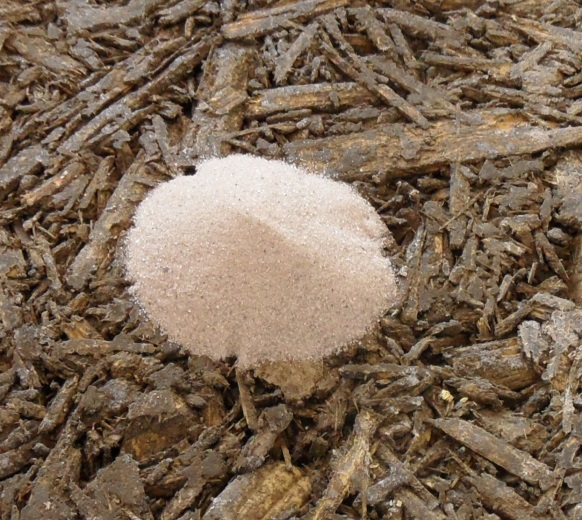
\includegraphics[width=7.7cm]{sandfleck.png}
	\caption{Aufgeschütteter Sandfleck}
	\label{sandfleck}
\end{minipage}
\hfill
\begin{minipage}[hbt]{7cm}
	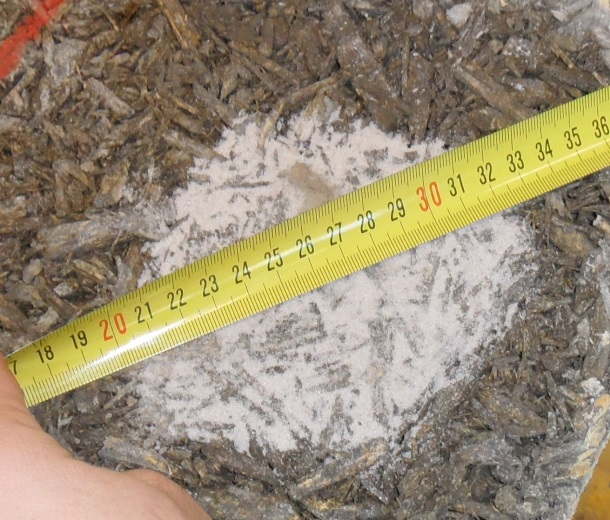
\includegraphics[width=8cm]{sandfleckmessen.png}
	\caption{Ermittlung des mittleren Durchmessers}
	\label{sandfleckmessen}
\end{minipage}
\end{figure}
\paragraph{Berechnng des Kleberbedarfs: SikaTop-109 ElastoCem, nach Sika}

\textbf{Angaben:}
\begin{center}

\begin{itemize}
\item mittlere Durchmesser:D=11$cm$
\item Sandvolumen:	V=0,01$L$
\item Dichte:	$\rho$=1.60 $\frac{kg}{L}$
\item Trägerabmessung(l x b):	7,40 x 0,50 $m $
\end{itemize}
\end{center}


\textbf{Annahmen:}

\begin{itemize}
\item Spachtelfaktor:	$sp=\dfrac{2}{3}$
\item Schichtdicke:		$sd=3mm$
\end{itemize}
 

\subparagraph{Berechnung der Rauigkeit:}
\begin{equation}
r=\dfrac{V*4}{\pi*d^{2}}=1,052 mm
\end{equation}

\subparagraph{Kleberbedarf/$m^{2}$}

\begin{equation}
Kb= 2\dfrac{kg}{L}*sd=6\dfrac{kg}{m^{2}}
\end{equation}

\subparagraph{Kleberbedarf für Porenverschluss: Kp}

\begin{equation}
Kp=r*\rho*sd= 1,122\dfrac{kg}{m^{2}}
\end{equation}

\subparagraph{Bedarf für CLT-Velox-Schichte}

\begin{equation}
B_{CLT-Velox}=Kb*l*b=22,22 kg
\end{equation}

\subparagraph{Bedarf für Velox-Velox-Schichte}

\begin{equation}
B_{Velox-Velox}=(Kb+Kp)*l*b=26,35 kg
\end{equation}


\subparagraph{Benötigter Kleber für den gesamten Träger}

\begin{equation}
B_{gesamt}=B_{CLT-Velox}+2*B_{Velox-Velox}=74,91 kg
\end{equation}




\subsection{1 Kleberversuchsreihe}

Beim 1 Großbauteilversuch, kam der Kleber Sikadur 31 zur Anwendung. Dieser Kleber wurde auch von Herrn Dipl.Ing. Kirchmayer bei seinen Verbundversuchen verwendet. Da der Aufbau von Herrn Kirchmayer kleiner war und somit auch die Klebermenge geringer, hatte er keine Probleme bei der der Verarbeitung. Der Kleber entwickelt bei großen Mischmengen eine schnelle Aushärtezeit und war beim Auftragen über den gesamten Träger sehr schwer zu Verarbeiten. Dies war auch bei der Ansicht, von Teilen des Versuchskörpers ersichtlich. In der Abbildung \ref{kleberfoto} sind gorße Flächen zu erkennen, auf denen keine oder nur geringe Spuren des Veloxmaterials haften blieb. Dies ist auf die ungenügende Verarbeitung zurückzuführen. Um den eine bessere Verarbeitung zu gewährleisten und wirtschaftlichere Kleber zu verwenden, wurden alternative Kleber untersucht. 
\begin{figure}[h]
\begin{center}
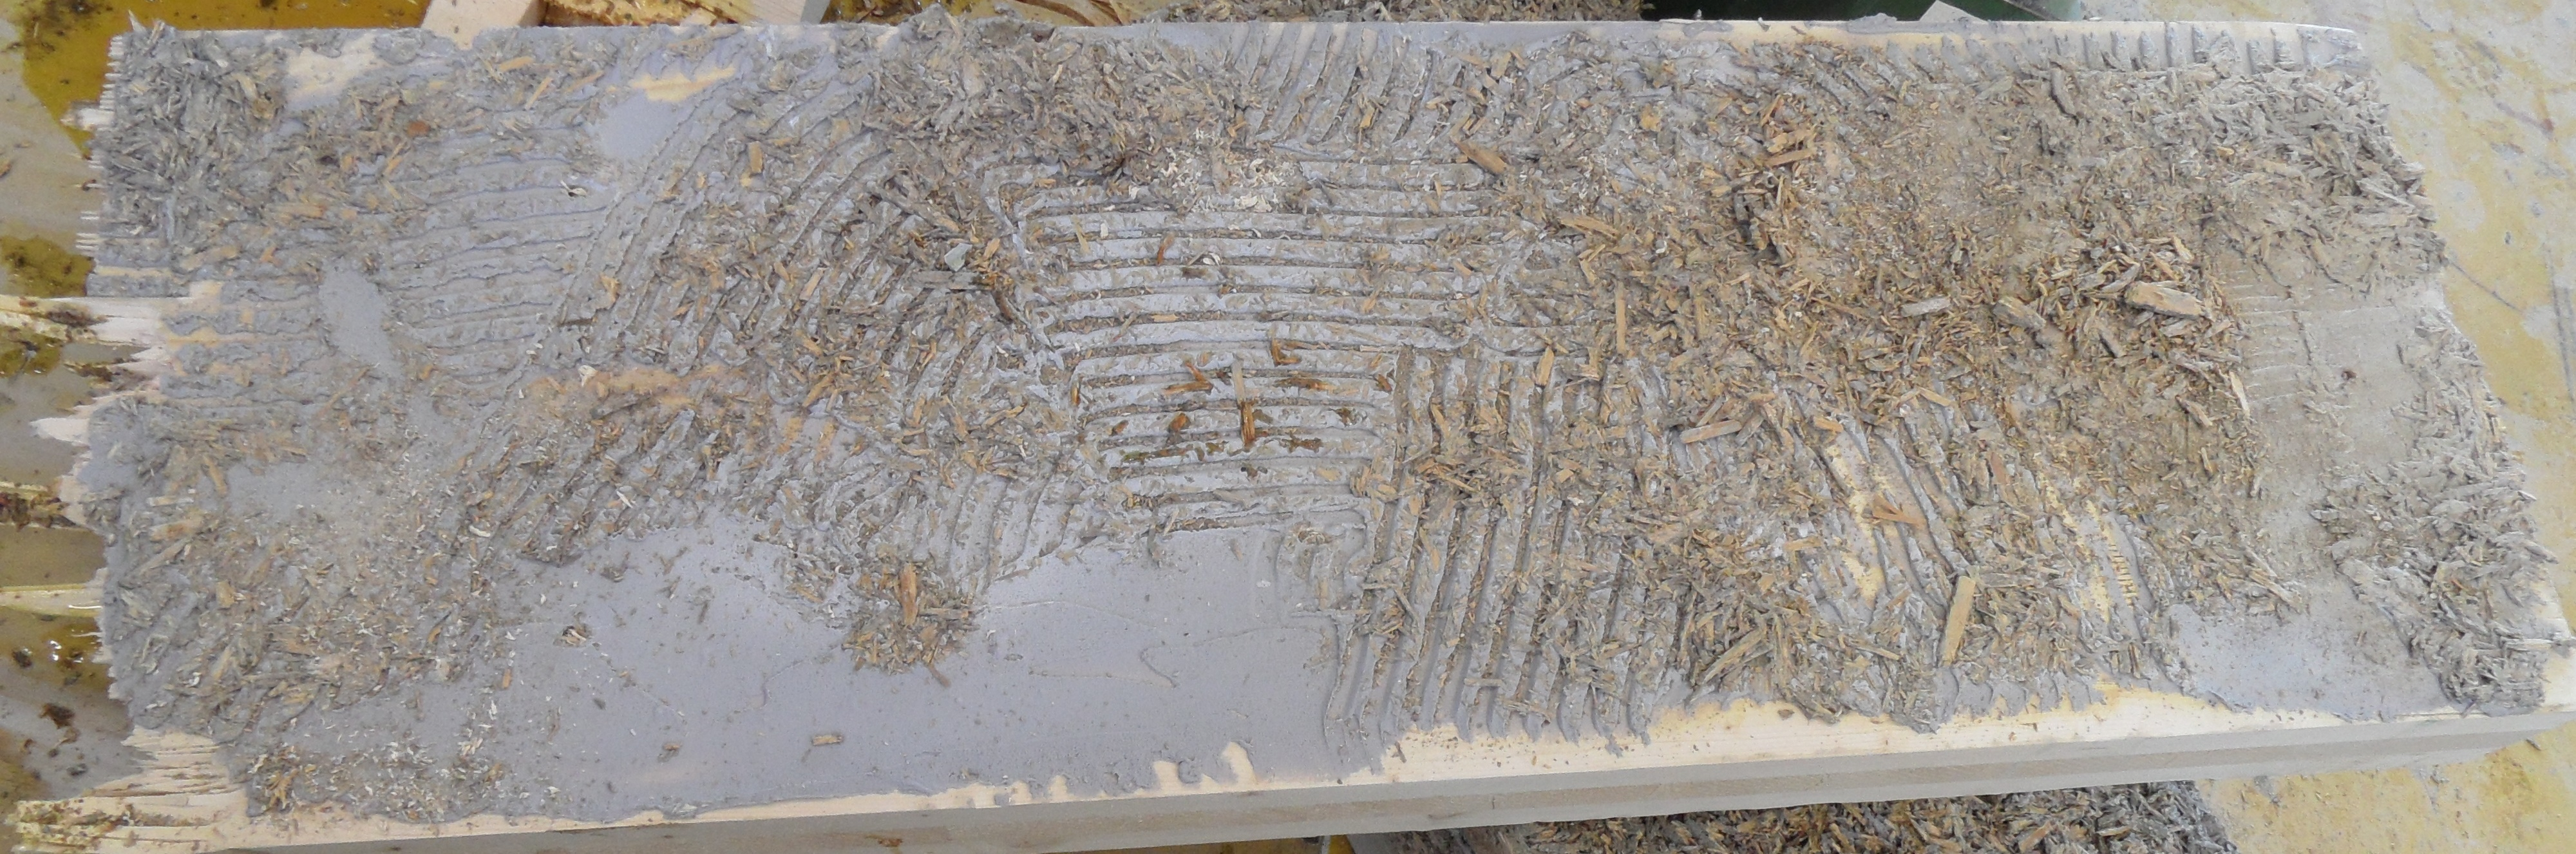
\includegraphics[scale =0.1]{kleberfoto.jpg}
\caption{ Verbundfäche von der Kleberschicht: CLT-Velox}
\label{kleberfoto}
\end{center}
\end{figure}



In Abstimmung mit der Firma Sika wurde die Anwendung abgeklärt und folgende Kleber getestet:
\begin{itemize}
\item Sikafloor 161
\item ElastoCem 109
\item SikaForce 7710 L35
\end{itemize}


auf folgende Eigenschaften der Kleber sind wir näher eingegangen :	

\begin{itemize}
\item Verarbeitbarkeit
\item Haftzug
\item Verbrauch
\end{itemize}


\textbf{ Anmischen:}
 Die Untersuchten Kleber bestanden alle aus dem 2 Komponenten-System. Daher mussten die Komponenten nach dem vom Hersteller  angegebenen Mischverhältnis abgemischt werden. Um eine einheitliche Masse zu erhalten mussten die 2 Komponenten mit einem Quirl gemischt werden, um eine einheitliche Klebermasse zu bekommen. Der Vorgang war bei allen Klebern ident. Der Kleber Sikafloor 161 wurde noch zusätzlich mit einem Thixotropierungsmittel verarbeitet, da er zu dünnflüssig war. Daher ergab sich ein erhöhter Aufwand bei der Vorbereitung.
\newline{}
\textbf{ Arbeitstechnik:}
Die Kleber wurden mit der Zahnspachtel vollflächig auf die Veloxplatte aufgetragen. 
Der Auftrag hatte sich einfach gestaltet, jedoch musste man mehrmals den Kleber verspachteln, um den Porenverschluss zu gewährleisten.
Bei der Vorbereitung für die Kleber ElastoCem 109 und Sikafloor 161 war nur auf das richtige Mischverhältnis zu achten. Der Kleberauftrag gestaltete sich einfach und schnell.
Beim Abfüllen des Klebers SikaForce 7710 L35 mussten wir vorsichtig sein, da der Kleber toxische Gase beinhaltet. Das Mischen der 2 Komponenten nicht schwierig. Der Auftrag des Klebers war wieder einfach und schnell.

\section{Haftzugprüfung}
Um den Verbund der Kleber mit der Veloxplatte zu Untersuchen, wurde die Haftzugprüfung angewendet.
Die Haftzugprüfung  wurde mit den angeführten Klebern durchgeführt. Zusätzlich wurde eine Prüfung ohne Kleber (nur auf das Velox) durchgeführt, um einen Referenzwert zu erhalten. In der Abbildung \ref{Z16E} ist das Prüfeinheit dargestellt.

\begin{figure}
\begin{center}
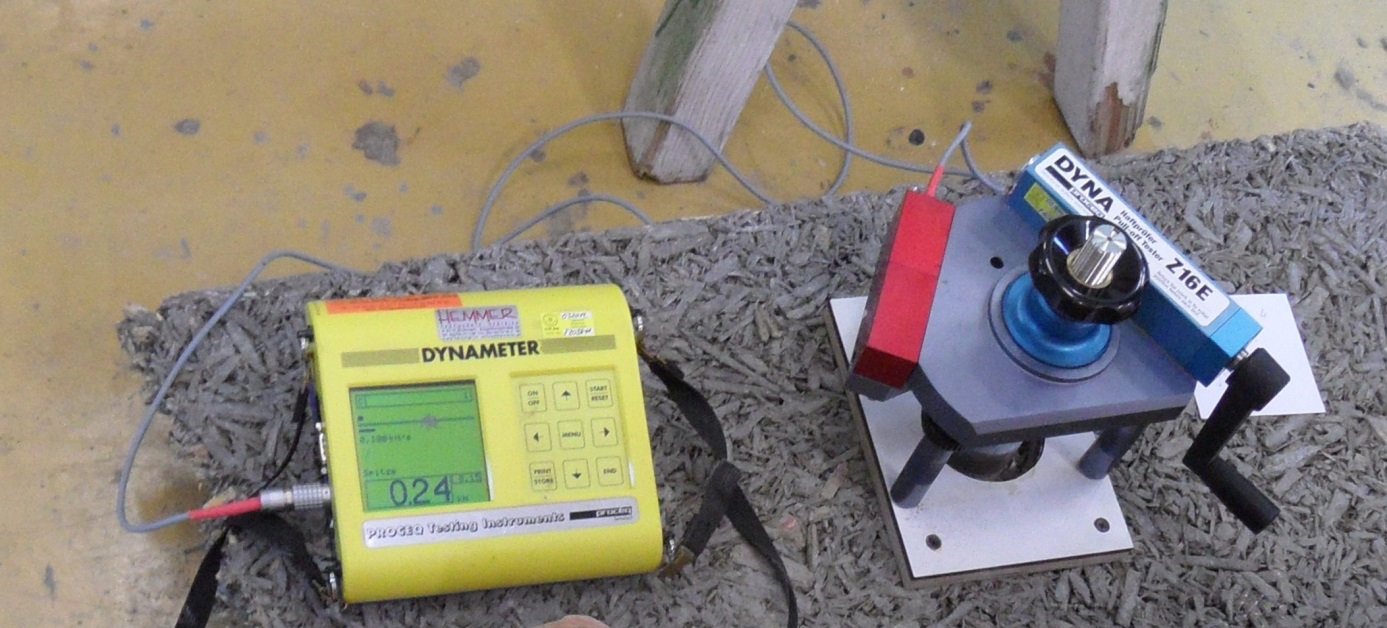
\includegraphics[scale =0.7]{Z16E.jpg}
\caption{ Prüfgerät:Dynameter Z16E}
\label{Z16E}
\end{center}
\end{figure}

\newpage{}

\subsection{Versuchsvorbereitung}

\begin{enumerate}
\item Anmischen des 2 Komponentkleber
\item Auftragen der Kleber auf das Velox.
\item Aushärtezeit:  1 Woche
\item 3 Kernbohrungen wurden auf jeden Versuchskörper aufgebracht
\item Aufwärmen der Prüfstempel (Beschleunigung der Aushärtung)
\item Abmischen des Klebers des Klebers für die Kraftübertragung zwischen dem Stempel und den Testkleber
\item Auftragen des Klebers (Uhuplus oder X60)
\item Aufbringen des vorgewärmten Prüfstempels
\item Aushärten des abgemischten Klebers (15 min oder 4 min)
\end{enumerate}

\newpage{}
In den nachfolgenden Abbildungen \ref{1Versuchsplatte} - \ref{4Versuchsplatte} sind die getrockneten Kleber und die aufgeklebten Prüfstempel ersichtlich.

\begin{figure}[h]
\begin{minipage}[hbt]{7cm}	
	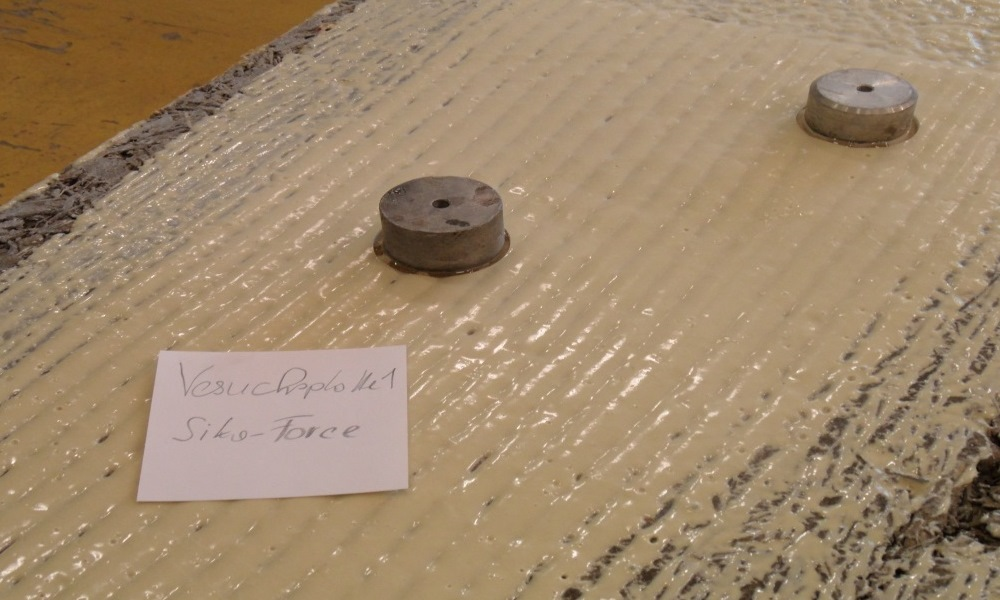
\includegraphics[width=7cm]{1Versuchsplatte.jpg}
	\caption{Versuchsplatte (Sika-Force 7710 L35)}
	\label{1Versuchsplatte}
\end{minipage}
\hfill
\begin{minipage}[hbt]{7cm}
	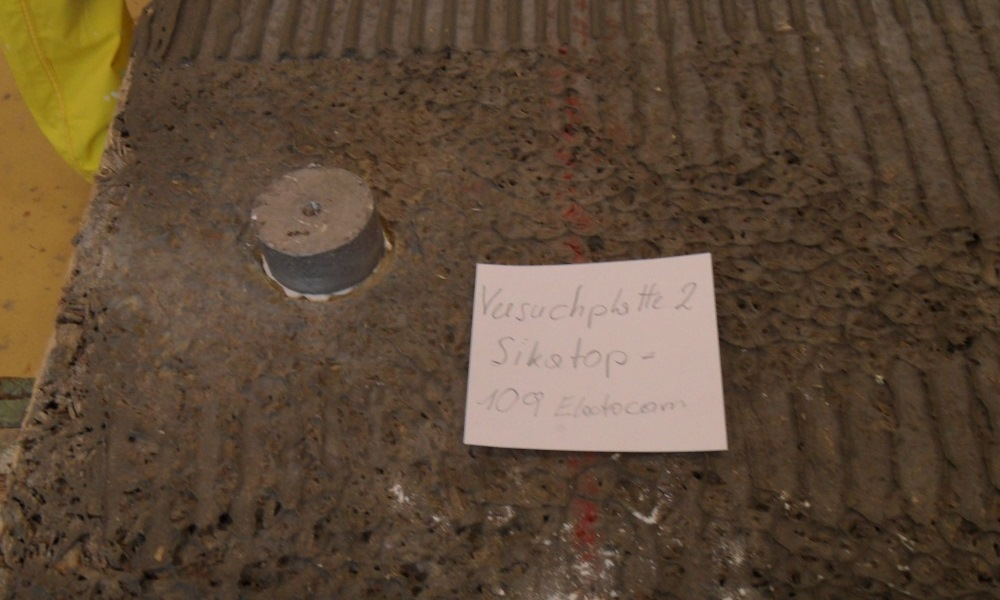
\includegraphics[width=7cm]{2Versuchsplatte.jpg}
	\caption{Versuchsplatte (Sikatop-109 Elastocam)}
	\label{2Versuchsplatte}
\end{minipage}
\end{figure}


\begin{figure}[h]
\begin{minipage}[hbt]{7cm}	
	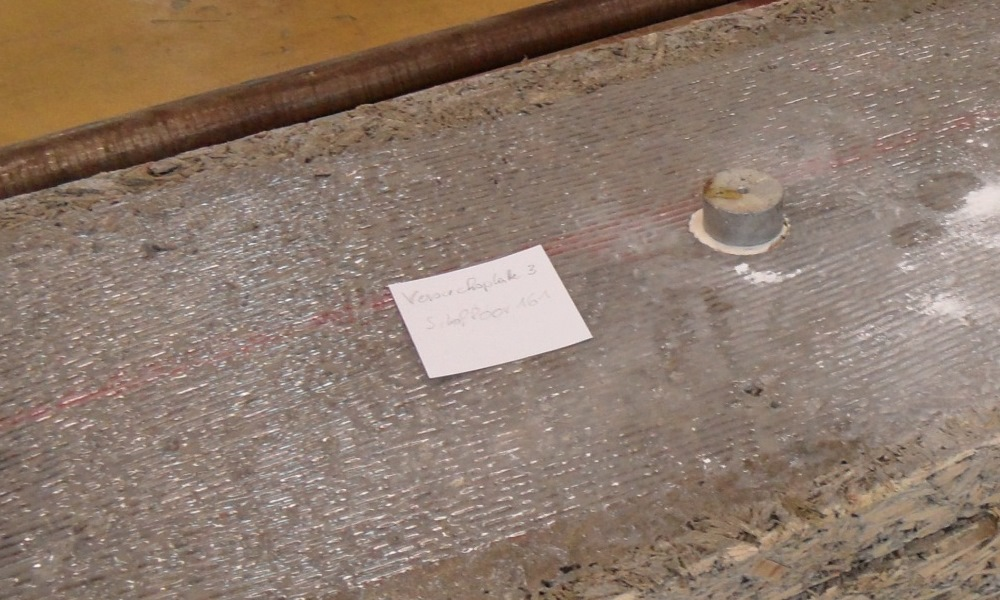
\includegraphics[width=7cm]{3Versuchsplatte.jpg}
	\caption{Versuchsplatte (Sikafloor 161))}
	\label{3Versuchsplatte}
\end{minipage}
\hfill
\begin{minipage}[hbt]{7cm}
	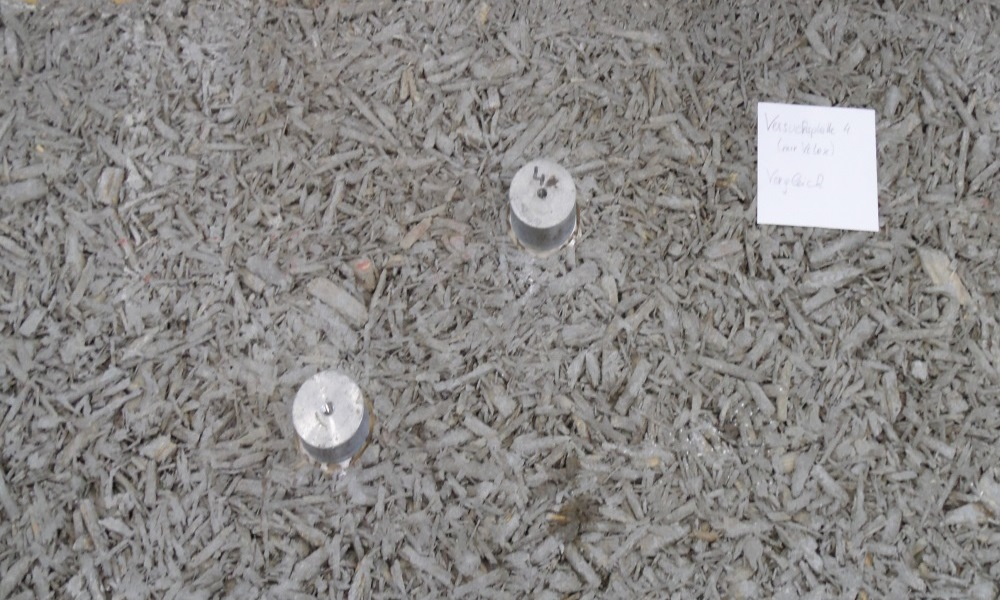
\includegraphics[width=7cm]{4Versuchsplatte.jpg}
	\caption{Versuchsplatte (ohne Kleber)}
	\label{4Versuchsplatte}
\end{minipage}
\end{figure}

\subsection{Versuchsdurchführung}

\begin{enumerate}
\item Einschrauben des Bolzens in den Stempel
\item Aufstellen des Haftzugprüfgeräts (Dynameter Z16E)
\item Einfädeln des Bolzens in die Einkerbung
\item manuelles Kraftaufbringen durch die Handkurbel
\item Ablesen der max. Kraft auf dem Messgerät
\end{enumerate}

In der Abbildung \ref{dynameter} ist die Messeinheit mit den beschrifteten Hauptbestandteilen dargestellt. 

\begin{figure}
\begin{center}
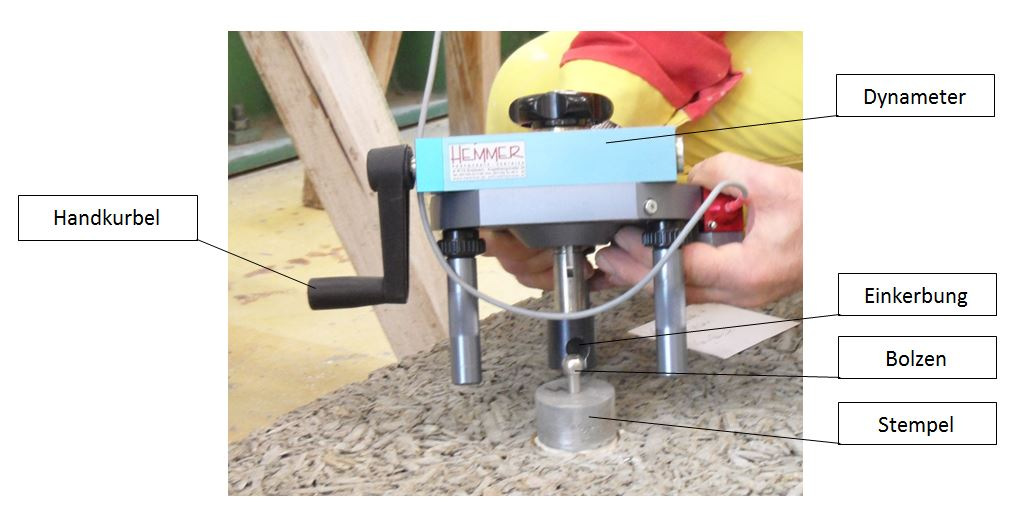
\includegraphics[scale =0.7]{dynameter.jpg}
\caption{ Erklärung des Prüfgeräts:Dynameter Z16E}
\label{dynameter}
\end{center}
\end{figure}



\begin{table}
\caption{Auswertung der 1 Kleberversuchsreihe}
\begin{center}

\begin{tabular}{|c|c|c|c|c|} \hline
Versuchsplatte & Kraft & Durchschnitt & Spannung &Durchschnitt \\\hline

	& [kN] & [kN] & [N/mm$^{2}$] & [N/mm$^{2}$] \\
	\hline\hline
 \cline{2-2} 1 Versuch: Sika Force  & 1,47 & & 0,75& \\\cline{2-2}&1,56 &1,45 &0,79 &0,74 \\\cline{2-2}&1,32 & &0,67 & 
\\\hline\hline

 \cline{2-2} 2 Versuch: Sikatop 109  & 0,74 & & 0,38& \\\cline{2-2}&0,77 &0,77 &0,39 &0,39 \\\cline{2-2}&0,80 & &0,41 & 
\\\hline\hline

 \cline{2-2} 3 Versuch: Sikafloor 161  & 2,11 & & 1,07& \\\cline{2-2}&1,82 &2,04 &0,93 &1,04 \\\cline{2-2}&2,20 & &2,12 & 
\\\hline\hline


 \cline{2-2} 4 Versuch: nur Velox  & 0,84 & & 0,43& \\\cline{2-2}&0.80 &0,82 &0,41 &0,42 
\\\hline

\end{tabular}
 \label{tab:1 kleberversuche}

\end{center}
\end{table}




\textbf{Zwischenfazit:}
\newline

Die Kleber bei den Versuche 1 und 3 haben sehr gute Klebeeigenschaft die man anhand der Versuchsergebnisse \ref{tab:1 kleberversuche} erkennen kann. Es versagte bei den beiden nicht der Kleber sondern das Velox. Die innere Festigkeit vom Velox war geringer, als die des Klebers. 

Beim 2 Versuch hat nicht das Velox versagt, sondern der Kleber. Es ist zu vermuten, dass das Velox eine höhere innere Festigkeit hat als der Kleber hat. Da der Kleber ElastoCem 109 auf Zementbasis agiert, ist eine Aushärtezeit von 28 Tagen erforderlich, damit er seine Endfestigkeit erreicht.  Somit werden die Ergebnisse der Haftzugprüfung nach einer Woche unterschätzt.  Die Haftzugfestigkeit wird im Produktdatenblatt der Fa. Sika mit 0,7 N/$mm^{2}$ geführt. Daher ist zu erwarten, dass die innere Festigkeit des Klebers mit längerer Aushärtezeit ansteigt.
Aufgrund der einfachen Vorbereitung und der guten Verarbeitung haben wir uns für den Kleber \textbf{Sikatop 109} für den Sandwichbauteil entschieden. Die innere Festigkeit sollte laut dem Produktdatenblatt[] nach entsprechender Aushärtezeit, höher als die die vom Velox sein. Durch die Verwendung des Aufbetons muss eine entsprechende Aushärtezeit für den Bauteil vorgesehen werden und ergibt daher die keine Einschränkung für den Kleber. 



\subsection{2 Kleberversuchsreihe}

Es wurden nach dem 2 Großbauteilversuch weitere Kleberversuche durchgeführt. Der Grund war, dass der Kleber ElastoCem 109 schon beim einheben in die Prüfeintichtung Beschädigungen aufwies. Es waren schon Teile der Veloxschichten nicht mehr miteinander verbunden. Dies war vor allem bei den Auflager ersichtlich. Durch den nicht vorhandenen Verbund waren auch Zugrisse in der Aufbetonschicht aufgetretten. In den Abildungen \ref{lagera} und \ref{lagerb} ist dargestellt, in welchen Ausmaß sich die Veloxplatten von einander lösten. Die Messlatte war 30 $ cm $ lang und die Unterteilungen kennzeichnen 5 $ cm $ Schritte.  

\begin{figure} [h]
\begin{minipage}[hbt]{7cm}	
	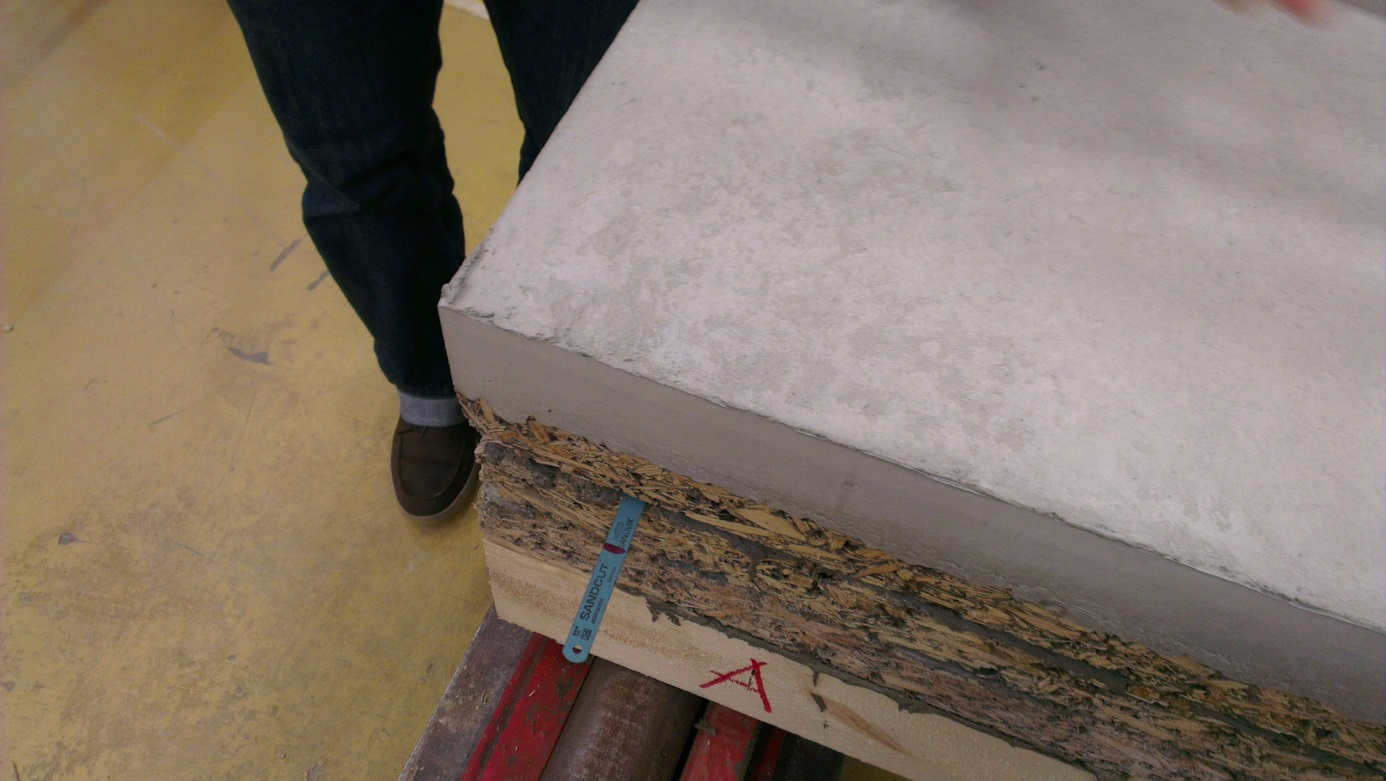
\includegraphics[width=7.7cm]{lagera.jpg}
	\caption{Verbundlosigkeit beim Auflager A}
	\label{lagera}
\end{minipage}
\hfill
\begin{minipage}[hbt]{7cm}
	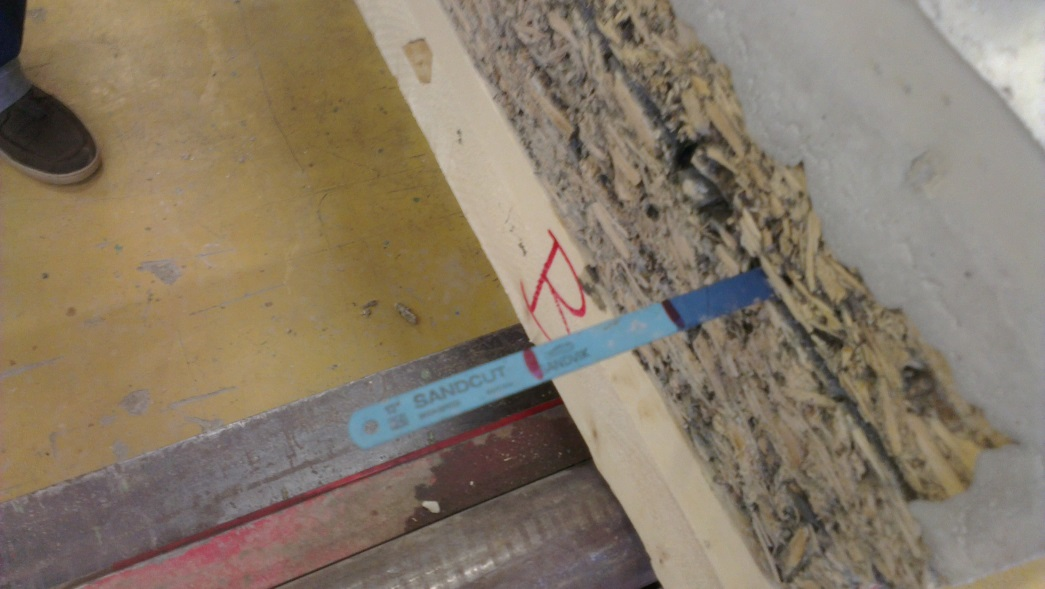
\includegraphics[width=8cm]{lagerb.jpg}
	\caption{Verbunglosigkeit beim Lager B}
	\label{lagerb}
\end{minipage}
\end{figure}



Es wurde wieder in der Absprache mit der Firma Sika ein  2 Komponenten Kleber auf Zementbasis gewählt SikaTop 107. Dieser Kleber hat  eine Doppel so hohe Festigkeit (lt.Produktdatenblatt[]) als der Kleber ElastoCem 109. Er besitzt die gleichen Verarbeitungsvorteile wie der Kleber ElastoCem 109.
 Um das Verbundverhalten des Klebers mit dem CLT-Holz zu untersuchen, wurden Versuchsproben erstellt. Der Aufbau und Ablauf des Versuch war genau gleich gestaltet wie der ersten Versuchsreihe.
In den Abbildungen \ref{holz-kleber} und \ref{velox-kleber} sind die Versuchskörper für das Clt (H1-H3) und für das Velox (V1-V3) dargestellt.


\begin{figure} 
\begin{minipage}[hbt]{7cm}	
	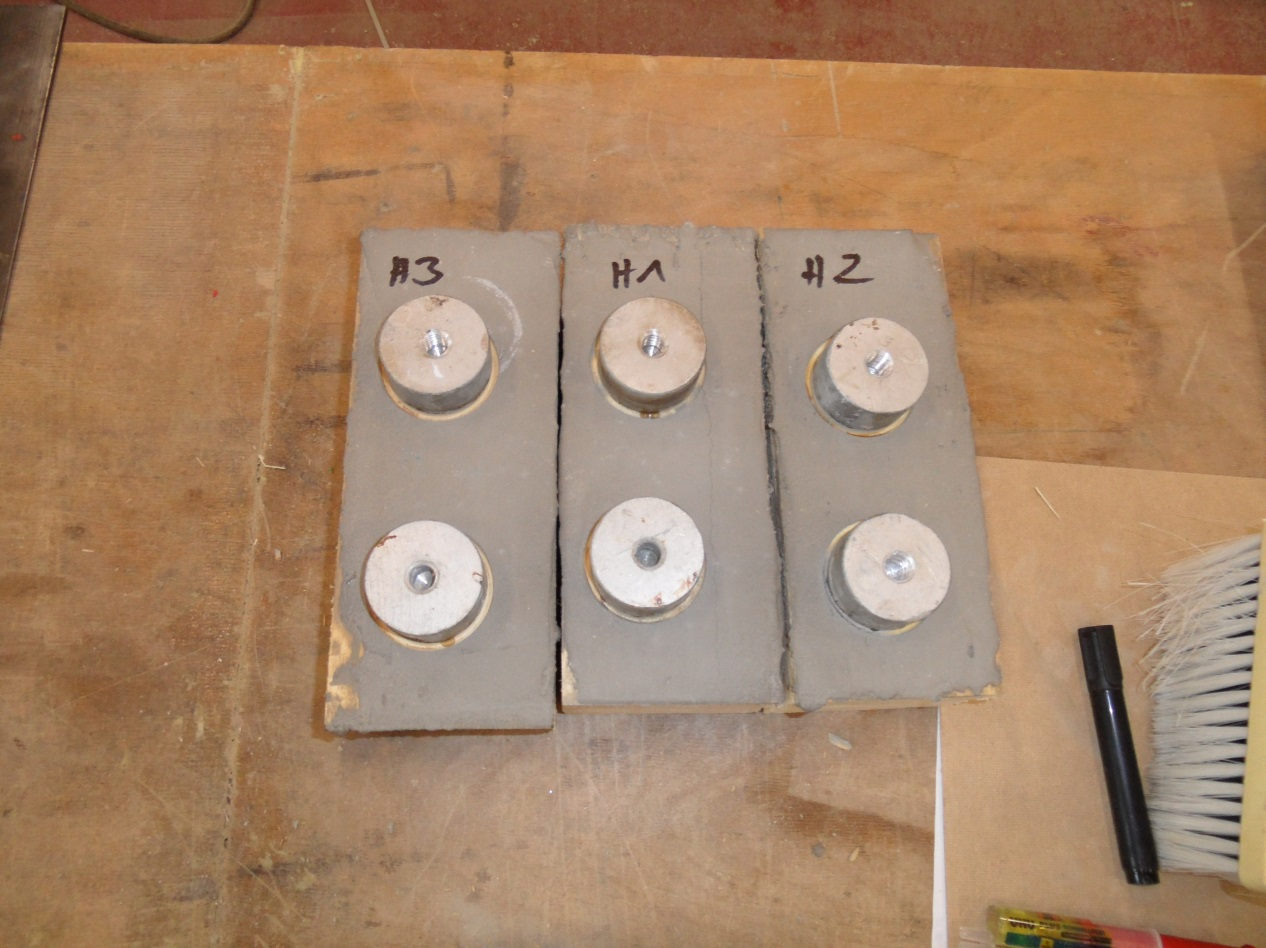
\includegraphics[width=7.7cm]{holz-kleber.jpg}
	\caption{Versuchskörper: Sikatop 107 auf Holz}
	\label{holz-kleber}
\end{minipage}
\hfill
\begin{minipage}[hbt]{7cm}
	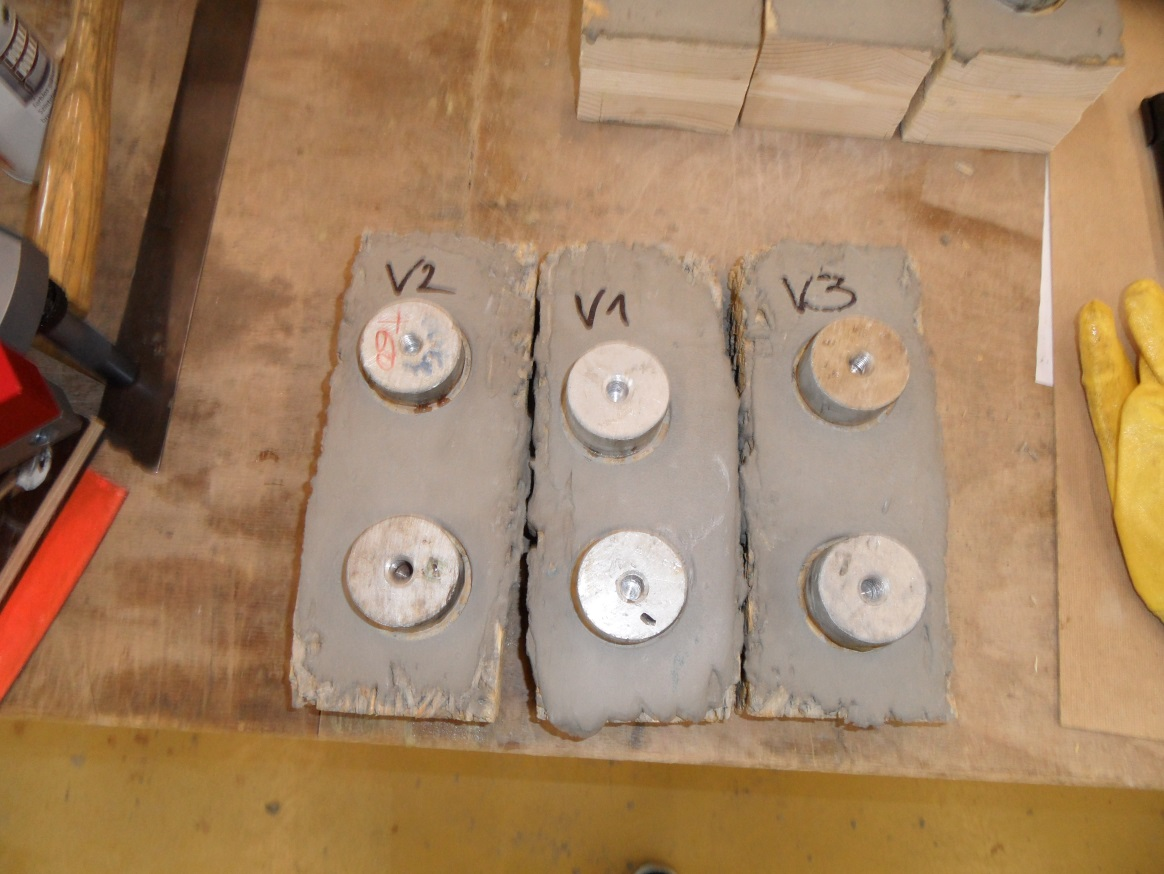
\includegraphics[width=8cm]{velox-kleber.jpg}
	\caption{Versuchskörper: Sikatop auf Velox}
	\label{velox-kleber}
\end{minipage}
\end{figure}

\paragraph{Allgemeines zum Versuch:}
Der Kleber Sikatop 107 wurde mit dem Mischverhältnis von 1:4,5 abgemischt und auf die Probenkörper aufgetragen. Vor dem Auftrag wurde das CLT Holz und das Velox noch befeuchtet, da beim aushärten des Klebers ein Feuchtigkeitstransport in das CLT-Holz stattfindet. Der Kleber hatte eine gleiche Aushärtezeit von einer Woche, um einen Vergleich zu der ersten Versuchsreihe zu erhalten. Der Ablauf der Haftzugprüfung erfolgte ident zu der 1 Kleberversuchen.

In der Abbildung \ref{probenbild} sind die Proben mit den dazugehörigen Oberflächen dargestellt. Einige Stempel weisen rot markierte Stellen auf, da in diesem Bereich der Kleber UHU-Plus nicht geklebt hat, \textbf{aufgrund von mangelnder Verarbeitung}. Daher wurden die Flächen um diesen Anteil abgemindert. [Tabelle:\ref{tab:2.1 kleberversuche}]

\begin{figure}
\begin{center}
\includegraphics[scale =0.8]{Probenbild.jpg}
\caption{Probendarstellung mit den markierten Stellen ohne Verbund}
\label{probenbild}
\end{center}
\end{figure}





\begin{table}
\caption{Auswertung der 2 Kleberversuchsreihe, CLT}
\begin{tabular}{|c|c|c|c|c|c|} \hline
\multicolumn{6}{|c|}{Sikatop auf CLT} \\\hline
Versuchsplatte & Kraft & Durchschnitt & Spannung & Abminderung & Durchschnitt \\\hline
	& [kN] & [kN] & [N/mm$^{2}$] & [\%] & [N/mm$^{2}$] \\
	\hline\hline
\cline{2-2} 1 Versuch: H1  & 1,25 & & 0,85& 25,0& \\\cline{2-2}&0.99 & 1,12 &1,51 & & 1,18
\\\hline\hline

\cline{2-2} 2 Versuch: H2  & 1,46 & & 1,30& 43,0& \\\cline{2-2}&1.86 & 1,66 &0,95 & & 1,13
\\\hline\hline

\cline{2-2} 3 Versuch: H3 & 1,07 & & 0,62&12,0 & \\\cline{2-2}&2,27 &1,67 &1,16 & 5,0 & 0,89 
\\\hline

\end{tabular}
 \label{tab:2.1 kleberversuche}
 \end{table}

\begin{table}
\caption{Auswertung der 2 Kleberversuchsreihe, Velox}
\begin{center}


\begin{tabular}{|c|c|c|c|c|} \hline
\multicolumn{5}{|c|}{Sikatop auf Velox} \\\hline
Versuchsplatte & Kraft & Durchschnitt & Spannung & Durchschnitt \\\hline
	& [kN] & [kN] & [N/mm$^{2}$] & [N/mm$^{2}$] \\
	\hline\hline
\cline{2-2} 1 Versuch: V1  & 0,34 & & 0,17&  \\\cline{2-2}&0.56 & 0,46 &0.30 &0,23
\\\hline\hline

\cline{2-2} 2 Versuch: V2  & 0,52 & & 0,26 &  \\\cline{2-2}&0,39 & 0,46 &0,20 & 0,23
\\\hline\hline

\cline{2-2} 3 Versuch: V3 & 0,26 & & 0,13 & \\\cline{2-2}&0,64 & 0,45 & 0,33 & 0,23  
\\\hline
\end{tabular}

\label{tab:2.2kleberversuche}

\end{center}
\end{table}


\newpage{}

\paragraph{Fazit:}

Bei der Betrachtung der Versuchsergebnisse ist eine markante Streuung der Ergebnisse bei den Velox ersichtlich. Betrachtet man den Versuch V3 dann sieht man eine Unterschied um mehr als das doppelte. Berechnet man jedoch einen Mittelwert, weichen die Werte kaum voneinander ab. Hier ist auch ersichtlich, dass bei jeder Probe die innere Festigkeit des Velox zu gering war. 
Um eine Aussage über den Verbund zwischen Kleber und CLT zu haben wurden diese ebenfalls getestet. Wie schon in der Anmerkung beschrieben, wurden die Ergebnisse noch korrigiert. Da die Ergebnisse mit der Flächen abgemindert worden sind, ist hier nur der Vergleich der Spannung aussagekräftig. Dieser Wert unterliegt auch einer Streuung von ca. 20 \%, wobei die Ergebnisse bei den beiden ersten fast ident sind. 
Wichtig war für uns, das nicht der Kleber bei den Versuch versagt sondern das Velox. Zusätzlich ist beim Vergleich der Ergebisse, dass die Spannungen beim Clt [Tabelle: \ref{tab:2.1 kleberversuche}] die Spannungen beim Velox [Tabelle:\ref{tab:2.2kleberversuche}] übersteigt.

\chapter{Aufbau des Großbauteilsversuch}

\section{Allgemeines}

Die durchgeführten Versuche unterschieden sich nur in der Verwendung von unterschiedlichen Verbindungsmittel. Es wurde zum einem die Anzahl der Schrauben variiert und zum anderen die mit unterschiedlichen Klebern experimentiert. Die Schichtenhöhe wurde nicht verändert, um die Auswirkungen der verschiedene Verbindungsmittel zu erkennen.

Der Schichtenabfolge und die Schichtenhöhe bzw. die Bauteilhöhe war bei allen Versuchen unverändert. In der Abbildung ist der Sandwichaubau \ref{sandwichaufbau} mit den verwendeten Dicken dargestellt.

\begin{figure}[h]
\begin{center}
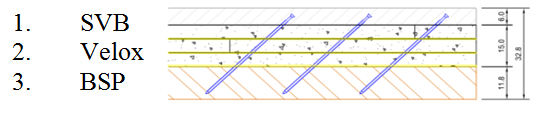
\includegraphics[scale =0.9]{sandwich.png}
\caption{Sandwichaufbau}
\label{sandwichaufbau}
\end{center}
\end{figure}



\section{Verwendete Bauteilkomponenten}
\subsection{Selbstverdichtender Beton, SCC}

Die Verwendung des SCC ist auf seine Vorteile zurückzuführen. Es ist ein besonders fließfähiger Beton, der sich selbst entlüftet und eine ebene Oberfläche bildet. Durch die Fließfähigkeit ist ein besonders guter Verbund mit dem porösem Werstoff,Holzbeton (Velox) gewährleistet. Die Betonschicht wurde auf eine minimale Dicke von 6cm reduziert. Das Limit ergibt sich aus der Verankerungslänge der Schrauben (4 $cm$)und der zuzüglich  Betondeckung von 2 $ cm $. Die Betonrezeptur hat Herr Dipl.Ing. Kirchmayer in den Versuchen ausgearbeitet und wurde von uns übernommen.


\begin{figure}[h]
\begin{center}
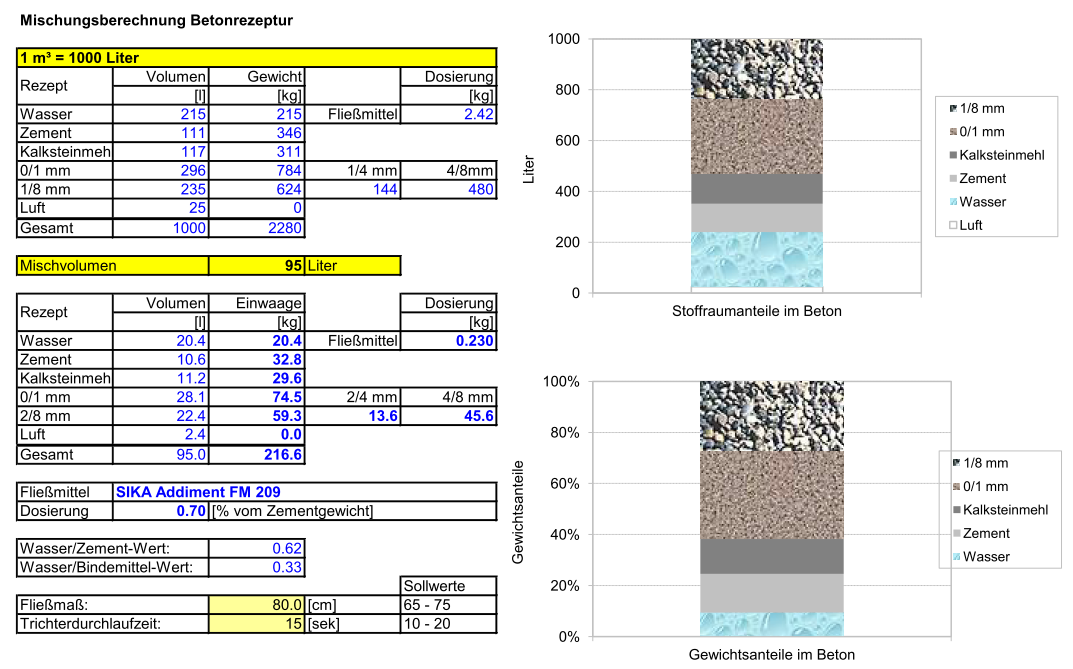
\includegraphics[scale =0.7]{Beton-Mischrezeptur.png}
\caption{Beton-Mischrezeptur [4], mit Okamurarechner}
\label{Beton-Mischrezeptur}
\end{center}
\end{figure}


\subsection{Holzspanbeton}

Holzspanbeton besteht aus den Komponenten Zement, Sägespänen, Wasser, und Additiven und eventuellen Zuschlagstoffen. Die Auswahl des Materials geht auf die Vorversuche von Herrn Kirchmayer bzw. Herrn Schernberger zurück. Die Verwendung der Veloxplatten stellte sich bei der Verarbeitung als sehr gut heraus. Jedoch muss erwähnt werden, dass bei den Versuchen zumeist das Velox versagt hat, und somit auch zusätzliche Verbindungsmittel angewendet werden müssen.
Die Abmessungen der Holzbetonschicht und der Holzplatte ergaben sich aus einem Vielfachen der Dicke der Velox-Platten (50 $mm$) und aus Vorberechnungen mit den FEM-Programm "Sofistik". Die Veloxplatte ist ein Industrieprodukt das ausführlich in der Ausarbeitung von Kirchmayer beschrieben wird.


\begin{figure}[h]
\begin{center}
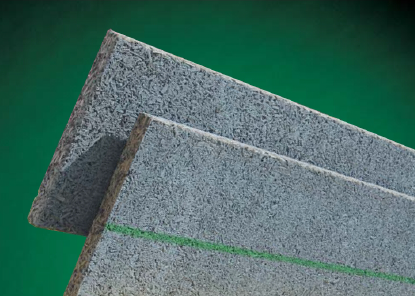
\includegraphics[scale =0.7]{velox.png}
\caption{Holzspanplatte WS 50 der Firma Velox}
\label{velox}
\end{center}
\end{figure}

\subsection{Kreuzlagenholz, CLT}

Die CLt-Platte ist ein flächiges Holzprodukt aus mindestens drei rechtwinkelig zueinander verleimten Schichten. CLT-Produkte zählen zu den Holzmassivbauweisen und können mit großen Abmessungen hergestellt werden. Aufgrund der Vorgabe die Spannweite 7,20m zu Überspannen wurde dieses Produkt gewählt. Es wurde auch schon in den Vorversuchen von Herrn Kirchmayer angewendet und gute Erfahrungen damit gemacht. Die Vorteile hat ebenfalls Herr Kirchmayer in seiner Arbeit schon ausgeabeitet.

Es wurde für alle Großbauteilversuche das Produkt BSP 118 3s DL ind. von der Mayr Mehlfhof  verwendet. In der Abbildung \ref{clt} ist ein Beispielbild einer 5 schichitgen CLT-Platte dargestellt.

\begin{figure}[h]
\begin{center}
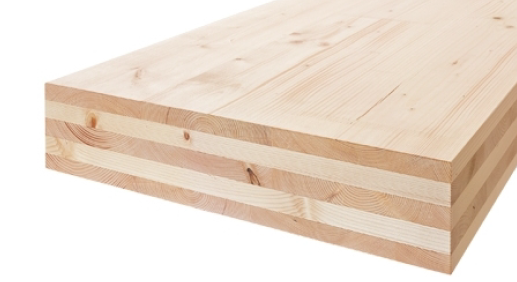
\includegraphics[scale =0.7]{clt.png}
\caption{5 - schichtige Brettsperrholzplatte (CLT)}
\label{clt}
\end{center}
\end{figure}

\subsection{Verbindunsmittel}

Um den Verbund der einzelnen Bauelemente herstellen zu können, kamen verschiedene Verbindungsmittel zur Anwendung. Aus den Vorversuchen von Kirchmayer ist hervorgegangen, dass die besten Verbundergebnisse durch Schrauben und Kleber  erzielt worden sind. Die Verbindungsmittel wurden von uns auch weiter verwendet.




\begin{itemize}
\item Schrauben
\newline
Die verwendeten Schrauben sind durch die Versuche ( siehe Kapitel 2.1) ausgewählt worden.
\newline
\begin{itemize}
\item SFS Intec WR-T-9x400
\end{itemize}

\item Kleber

Die angeführten Kleber im Kaptitel 2.2 Vorversuche beschrieben.
\newline

\begin{itemize}
\item Sikadur-31 AUT Normal Komp. B
\item ElastoCem-109 
\item Sikatop 107 
\end{itemize}

\end{itemize}

\section{Herstellung des Sandwichaufbaus}


\begin{figure}[h!]
	\begin{minipage}[h]{7cm}	
	 Die Herstellung der Versuchskörper war bei allen Proben ident. Wie schon angesprochen 	waren die Verbindungsmittel unterschiedlich angeordnet oder ausgeführt.
	Zu Beginn der Arbeiten haben wir alle Bauteilkomponenten bereitgelegt. Der 					zweikomponenten Kleber wurde mit dem Mischverhältnis, das vom Hersteller angegeben 			wird, abgemischt. Die erste Kleberschicht wurde auf die CLT-Platte aufgetragen. Der 		Auftrag erfolgte mit einer  8 $mm$ Zahnspachtel. Für die Verarbeitungszeit des Klebers 		war laut Datenblatt 45 min Topfzeit vorgegeben. Auf die Kleberschicht wurden die 			Veloxplatten aufgelegt. Dieser Vorgang wiederholte sich zwei mal, um auf die 				vorgegebene Schichtdicke zu kommen
	\end{minipage}
		\hfill
	\begin{minipage}[h]{7cm}
		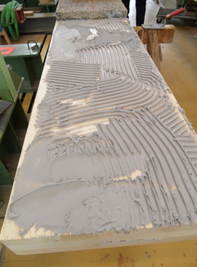
\includegraphics[width=7cm]{kleberauftrag.png}
			\caption{Kleberauftrag auf die CLT-Platte}
			\label{kleberauftrag}
	\end{minipage}
\end{figure}



\begin{figure}[h!]
\begin{minipage}[h]{7cm}
	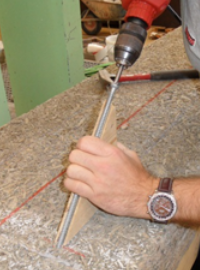
\includegraphics[width=7cm]{einschrauben.png}
	\caption{Einschrauben der Schrauben}
	\label{einschrauben}
\end{minipage}
\hfill
\begin{minipage}[h]{7cm}
Im nächsten Schritt wurde anhand des zuvor angefertigte Bohrmusters auf die obere Veloxschicht gekennzeichnet. Die Schrauben wurden mit einem Hilfswinkel und einem Hammer angesetzt um die geforderten 45 einzuhalten. Die Schrauben wurden anschließend ohne Vorbohren mit einer Bohrmaschine in den Bauteil eingebohrt. Um den Verbund mit dem Beton zu erhalten, stehen die  Schrauben 4 aus dem der oberen Veloxschicht heraus. Dieser Schritt wurde bei dem Bauteil ohne Schrauben nicht gemacht
	
\end{minipage}
\end{figure}

\begin{figure}[h!]
\begin{minipage}[h]{7cm}	
	Der letzte Schritt vor dem betonieren war, dass anbringen der Schalung. Es wurden Schalungsbretter auf eine Höhe von 20 $cm$ zugeschnitten. Die Schalung wurde mit einem Überstand von 6 $cm$ über der letzten Veloxschicht angebracht. Damit man den Überstand allseite gleich erhält, haben wir uns zwei Holzstücke mit den geforderten 6 $cm$ gefertigt. Somit hatte sich das Einrichten der Bretter, einfach gestaltet.  Die Bretter wurden mit Schrauben, die in die Veloxschicht eingeschraubt worden sind, befestigt. Durch die Befestigungsart der Schalung, war das Ausschalen des Trägers mit geringer Arbeit verbunden.

\end{minipage}
\hfill
\begin{minipage}[h]{7cm}
	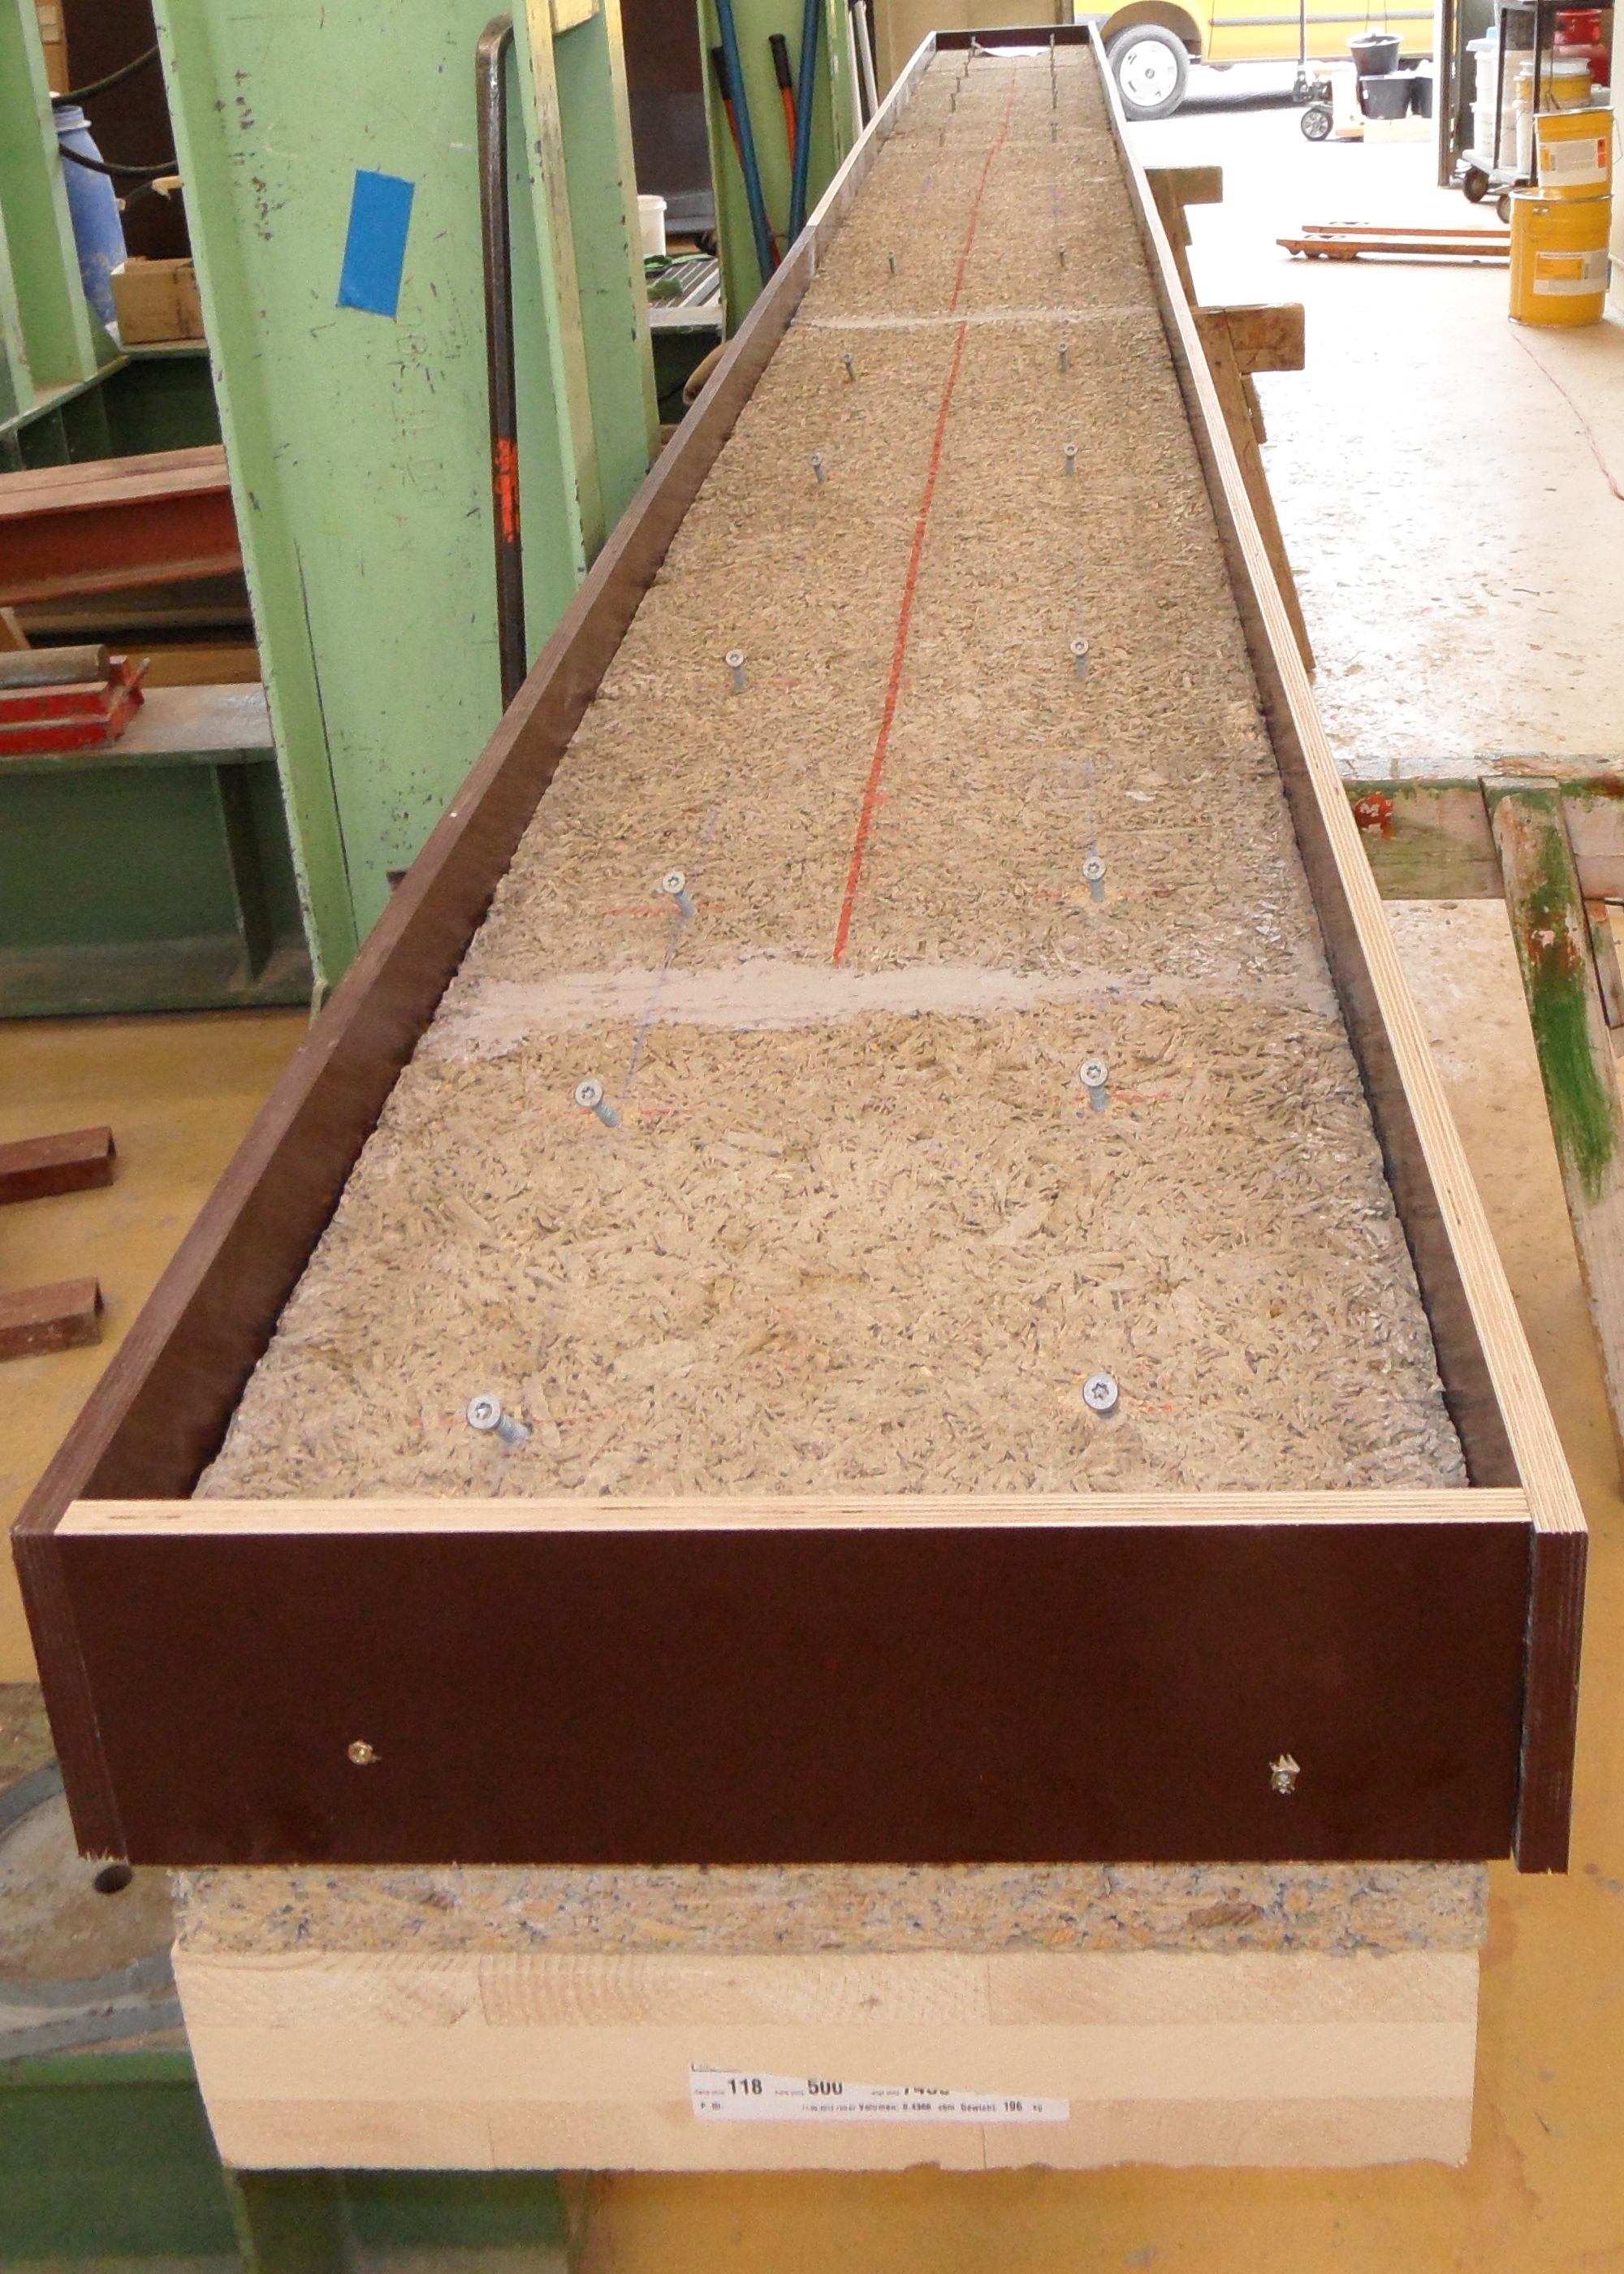
\includegraphics[width=7cm]{einschalen.png}
	\caption{Befestigung der Schalung}
	\label{einschalen}
\end{minipage}
\end{figure}


\begin{figure}[h!]
\begin{minipage}[h]{7cm}
	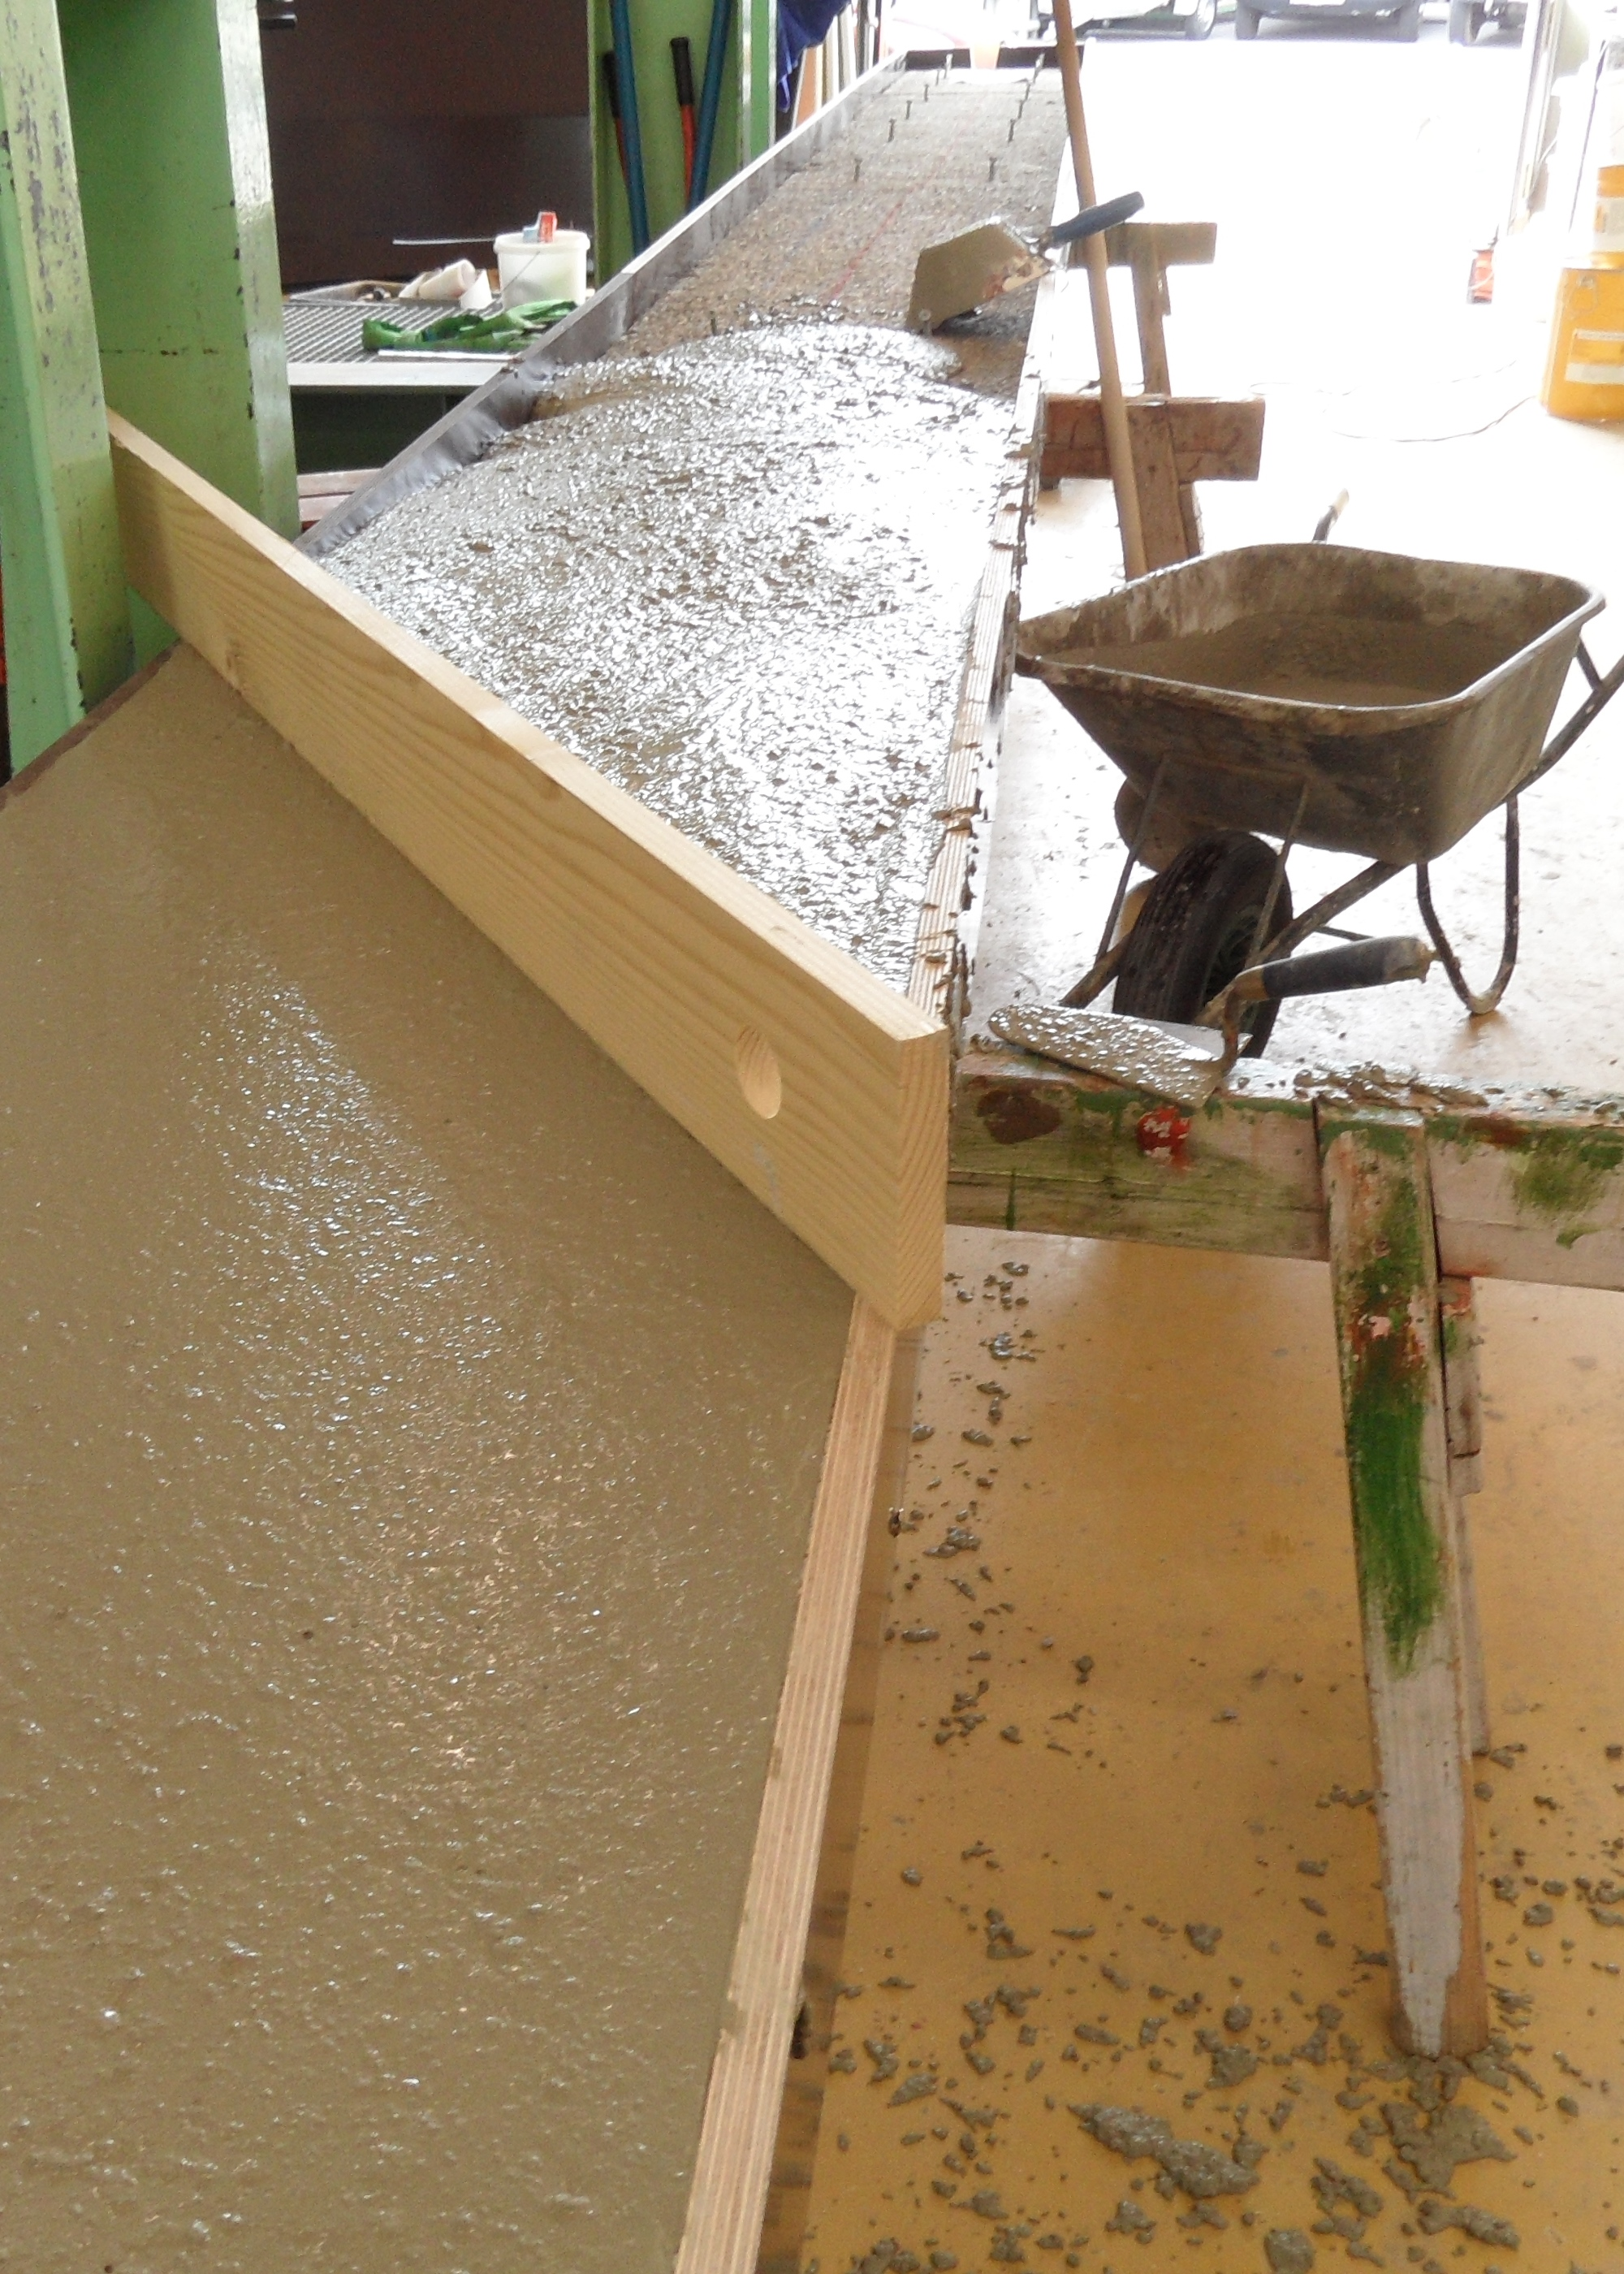
\includegraphics[width=7cm]{betonieren.png}
	\caption{Aufbrinden des SCC}
	\label{betonieren}
\end{minipage}
\hfill
\begin{minipage}[h]{7cm}
Abschließend wurde der Beton hergestellt. Die einzelnen Bestandteile wurden nach der Betonrezeptur [Abbildung: \ref{Beton-Mischrezeptur}] exakte eingewogen und danach mit einem Zwangsmischer vermischt. Der Beton wurde von Hand aufgebracht. Zum Schluss wurde der Beton mit einer Latte abgezogen und mit einem Schwert geglättet.
Für die Lagerung wurden 2 Böcke verwendet, die in den $1/4$ Punkten des Trägers angeordnet worden sind.

	
\end{minipage}
\end{figure}


\chapter{Versuchsaufbau und Durchführung}
Der Versuchsaufbau und die Abmessungen waren bei allen Versuchen wie in der Abbildung \ref{versuchsaufbau} dargestellt.Es handelt sich um einen 4-Punkt-Biegeversuch.   
Beim 4-Punkt-Biegeversuch wird die Prüfprobe auf 2 Auflagen (rote Dreiecke) positioniert und in den $1/4$  Punkten mit der Kraft (F) belastet. Der Vorteil besteht darin, dass zwischen den beiden Krafteinleitungspunkten ein konstantes Biegemoment herrscht. Der Versuchsaufbau ist einfach und er bildet die reale Belastung (Flächenlast) am besten ab. 

\begin{figure}[h]
\begin{center}
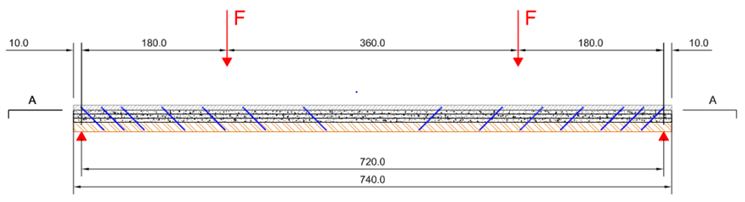
\includegraphics[scale =0.8]{versuchsaufbau.png}
\caption{Versuchsaufbau mit Lagerung und Lasteinleitung}
\label{versuchsaufbau}
\end{center}
\end{figure}

\section{Verwendete Messmittel und deren Anordnung}

Bei dem ersten und zweiten Großbauteilversuch wurde die Verschiebung noch manuell von den Messuhren abgelesen. Bei den Versuchen 3 und 4 wurde Messaufnehmer verwendet, die anschließend beschrieben werden. Die Aufnahme der Verschiebung erfolgte bei allen Versuchen an der gleichen Stelle. Die Messaufnehmer für die Trägerdurchbiegung,wurden in der Trägermitte und unter der Lasteinleitung angeordnet. Weiters wurde auf beiden Trägerenden Messaufnehmer angebracht, um die Verschiebung zwischen Betonschicht und der CLT-Schicht zu messen.

\begin{figure}[h]
\begin{center}
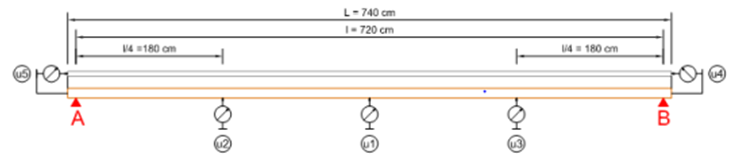
\includegraphics[scale =0.8]{messanordnung.png}
\caption{Anordnung der Messpunkte}
\label{versuchsaufbau}
\end{center}
\end{figure}

In der Abbildung \ref{versuchsaufbau} sind die Messpunkte skizziert und beschriftet.

\begin{figure}[h]
\begin{minipage}[hbt]{8cm}
	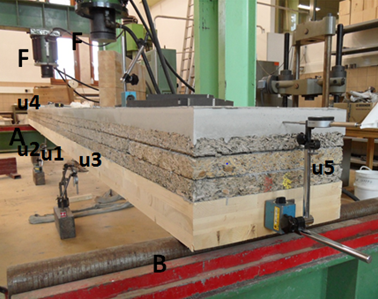
\includegraphics[width=8cm]{messpunkte.png}
	\caption{Mess- und Auflagerpunkte}
	\label{messpunkte}
\end{minipage}
\hfill
\begin{minipage}[hbt]{7cm}
	\begin{itemize}
	\item u1.1/ u1.2: Durchbiegung in Feldmitte 	auf beiden Seiten des Trägers
	\item u2/u3: Durchbiegung bei l/4
	\item u4/u5: Verschiebung der Betonschicht 	gegenüber der Holzschicht an beiden 	Enden des Trägers
	\item u4/u5: Krafteinleitung F ist im l/4 Punkt
	\item A/B Stellen bezeichnend die 	Auflagerpunkte 
	\end{itemize}

	
\end{minipage}
\end{figure}

\section{Wegaufnehmer}	

In diesem Abschnitt werden die die verschiedenen Wegaufnehmer beschrieben.

\subsection{Analoge Wegaufnehmer}

Es wurden analoge Messuhren von der Fa. Käfer verwendet. Die Messuhren besaßen einen Messweg von 7 $cm$ und haben eine Messgenauigkeit von $1/100  mm$. Die Vorrichtung für die vertikale Verschiebung, wurde mit einem Standfuss ausgeführt. Auf den Standfuss wurden die magnetischen Halteeinrichtungen angebracht, welche die Messuhren in der vorgesehenen Position hielten. Der gesamte Aufbau ist in dder Abbildung \ref{messuhr_unten} dargestellt.

Die Befestigung für die horizontale Verschiebung, wurde ebenfalls mit der magnetischen Halteeinrichtung bewerkstelligt. Zuvor musste noch eine Stahlplatte an der CLT-Platte angeschraubt werden, damit die Halteeinrichtung angebracht werden konnte. Der gesamte Aufbau kann der Abbildung \ref{messuhr_seitlich} entnommen werden.

\begin{figure}
\begin{minipage}[h]{6cm}
	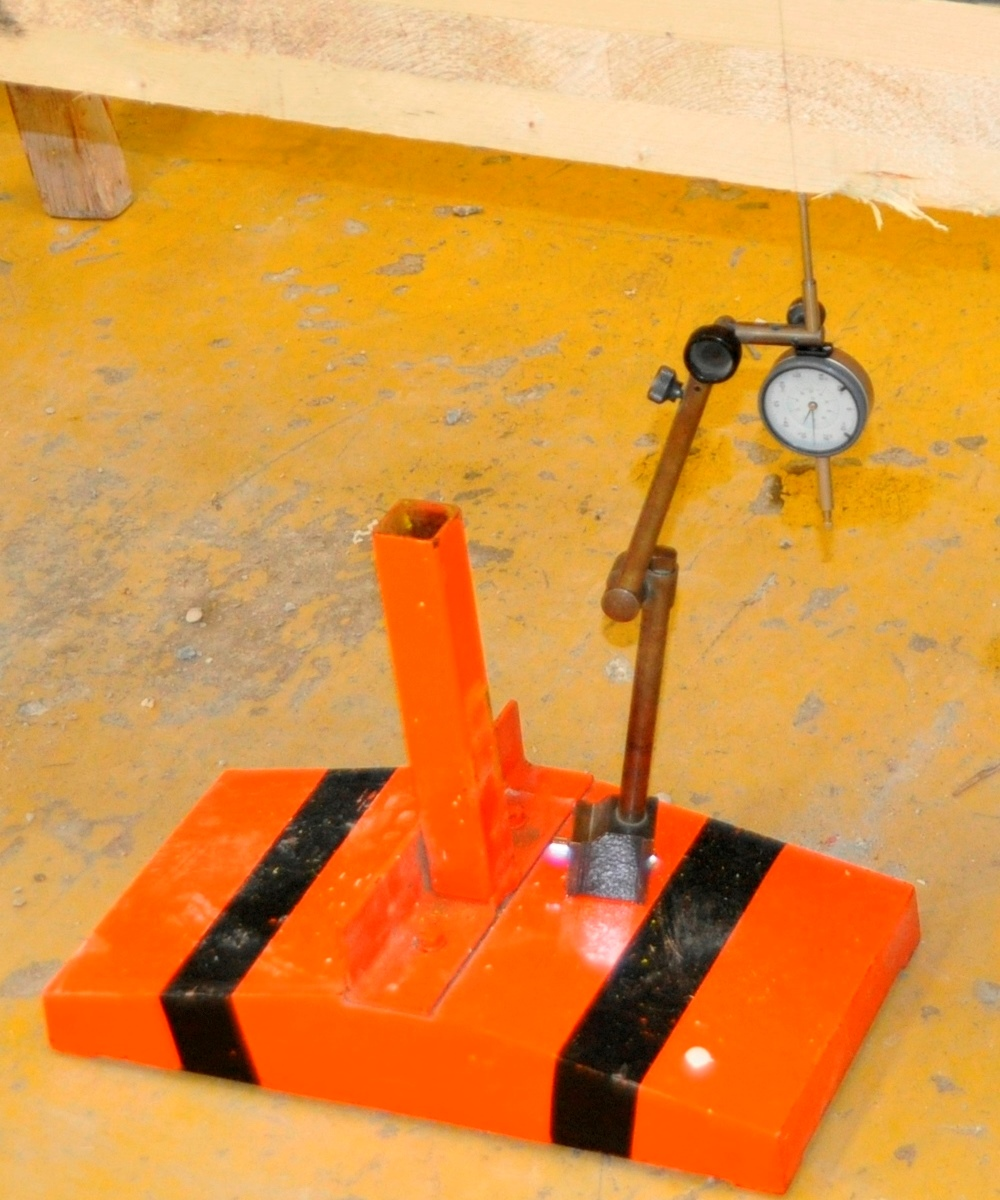
\includegraphics[width=6cm]{messuhr_unten.jpg}
	\caption{Messuhr für vertikale Verschiebung}
	\label{messuhr_unten}
\end{minipage}
\hfill
\begin{minipage}[h]{7cm}
	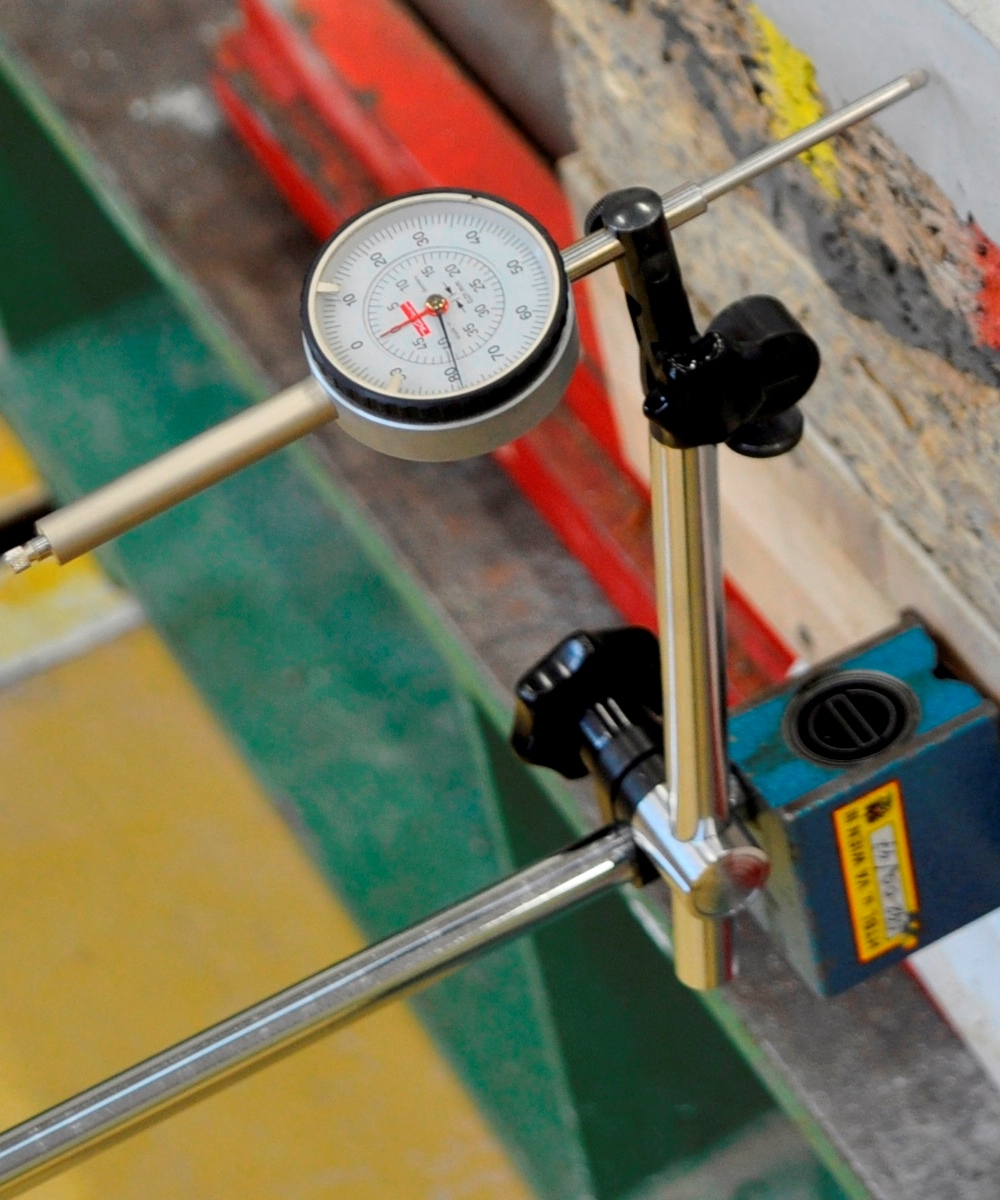
\includegraphics[width=7cm]{messuhr_seitlich.jpg}
	\caption{Messuhr für horizontale Verschiebung}
	\label{messuhr_seitlich}
\end{minipage}
\end{figure}


\subsection{Digitale Wegaufnehmer}

Es wurden digitale Seilzug Wegsensor von der Fa. MICRO-EPSILON verwendet[Serie WDS, Baureihe P60, 1000mm]. Die Messuhren besaßen einen maximalen Messweg von 100 $cm$ und haben eine Messgenauigkeit von $0,024  mm$. Die Vorrichtung für die vertikale Verschiebung, wurde ebenfalls mit dem Standfuss ausgeführt.In den Standfuss wurde die dazugehörige Metallstange eingeführt und mit kleinen Holzkeilen fixiert. Der  Wegsonsor wurde mit M4 Schrauben, Flügelmuttern und einer Holzplatte an der Metallstange montiert. Um das Seil auf der Messposition zu halten wurde eine Schraube in die CLT-Platte eingeschraubt. Der gesamte Aufbau ist in der Abbildung \ref{d_aufnehmer_unten} dargestellt.

Für die Messung der horizontalen Verschiebung, wurde eine Vorrichtung zusammengeschweißt. Die Vorrichung musste nur noch mit Schrauben auf der CLT-Platte angeschraubt werden. Der Wegsensor wurde ebenfalls mit M4 Schrauben, Flügelmuttern und einer Holzplatte, an der Vorrichung befestigt. Der gesamte Aufbau kann aus der Abbildung \ref{messuhr_seitlich} entnommen werden.



\begin{figure}[h!]
\begin{minipage}[h!]{5cm}
	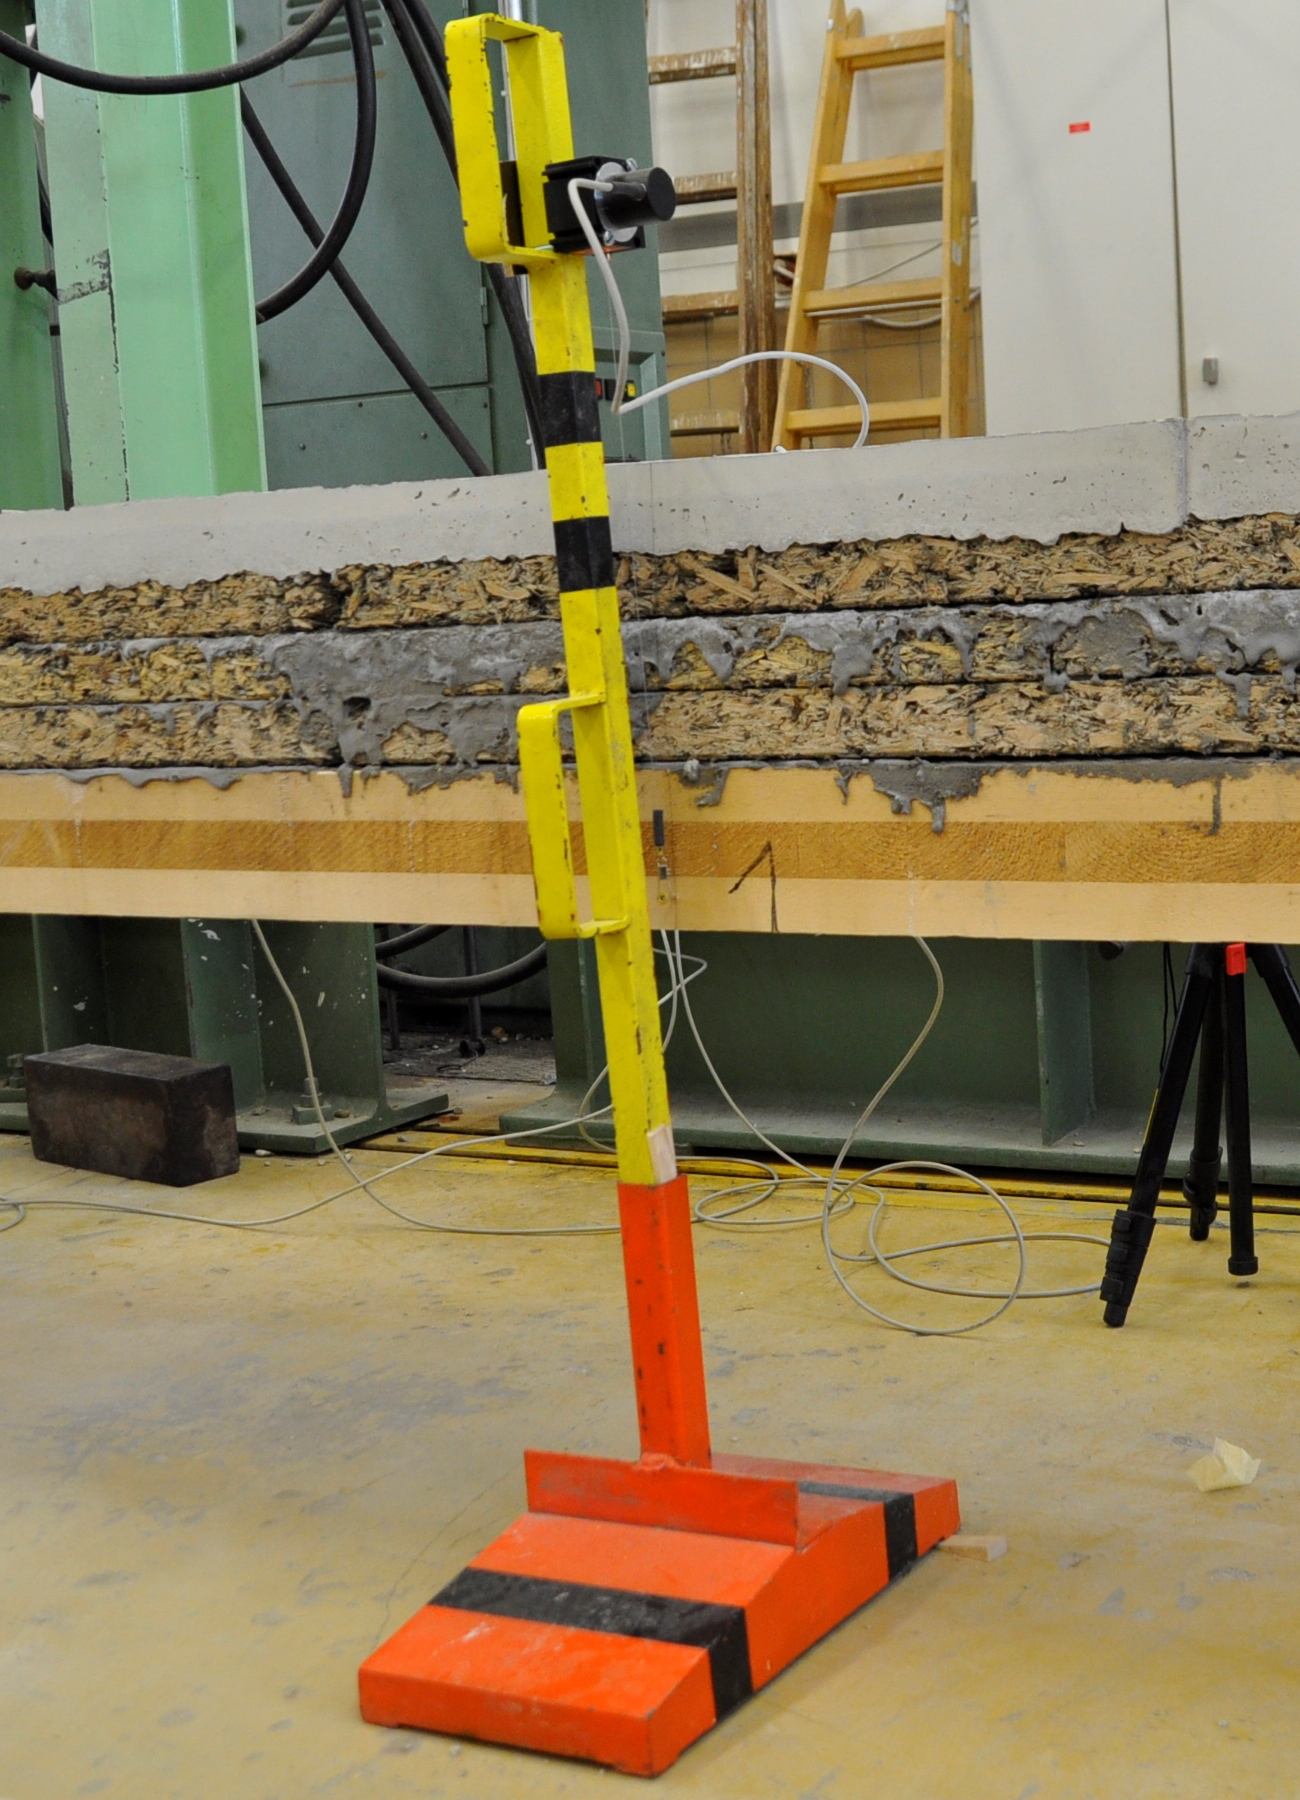
\includegraphics[width=5cm]{d_aufnehmer_unten.jpg}
	\caption{Messaufnehmer für vertikale Verschiebung}
	\label{d_aufnehmer_unten}
\end{minipage}
\hfill
\begin{minipage}[h!]{5cm}
	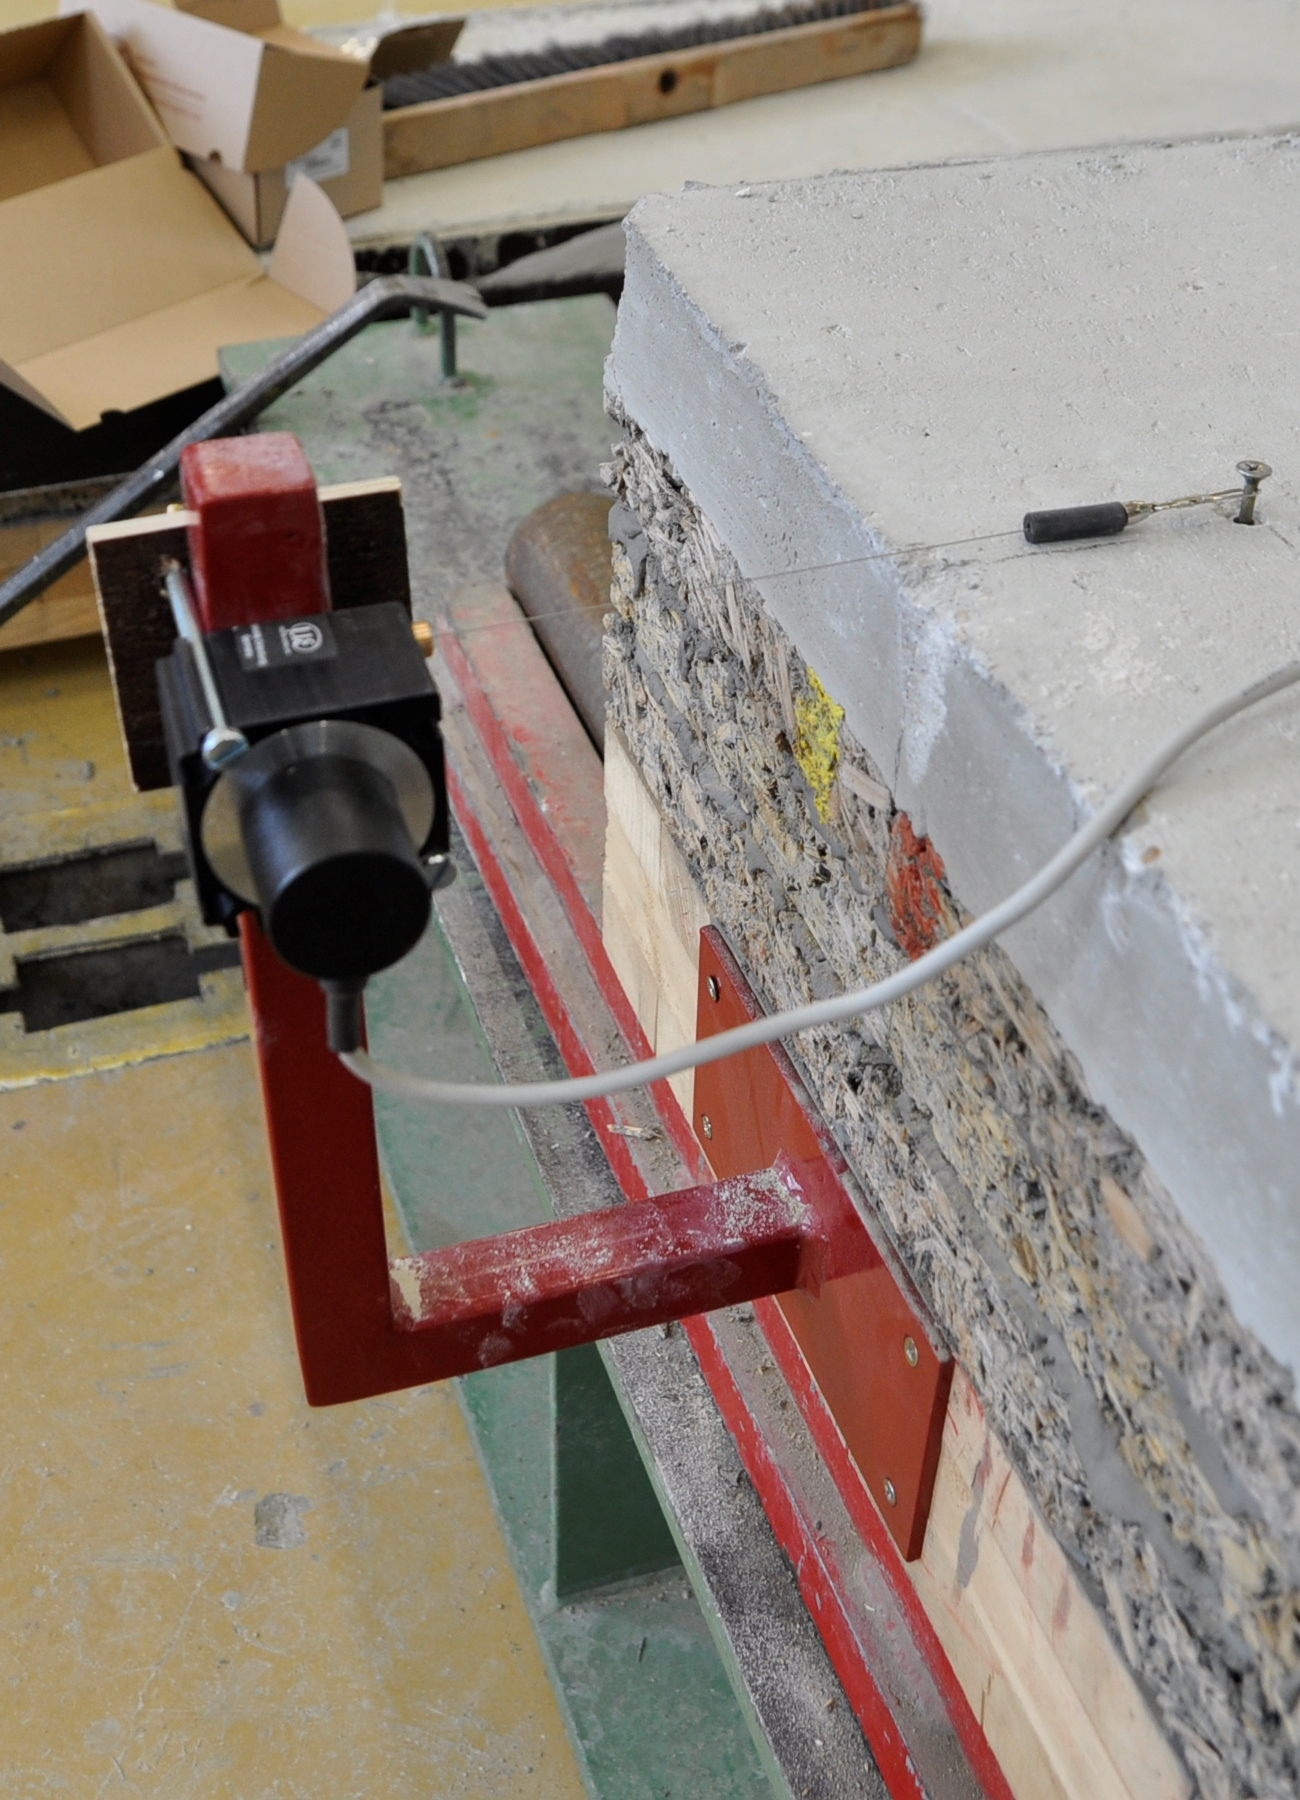
\includegraphics[width=5cm]{d_aufnehmer_seitlich.jpg}
	\caption{Messaufnehmer für horizontale Verschiebung}
	\label{d_aufnehmer_seitlich}
\end{minipage}
\end{figure}










	
\section{Durchführung des Versuchs}
Es wurde ein Versuch an einem Einfeldträger mit 4 Punkt Biegeverfahren durchgeführt. Die Lasteinleitung befand sich im viertel Punkt des Trägers, in der Mitte der Trägerbreite. Der Aufbau des Versuchs bzw. die Abmessungen des Bauteils ist in der Abbildung \ref{versuchsaufbau} zu entnehmen. Die Belastungsgeschwindigkeit für die Bauteilversuche 1 und 2 wurde mit 4 $kN/min$ gewählt.Das Ablesen erfolgte in Schritten von 2$kN$. Bei den Bauteilversuchen 3 und 4 wurde eine vorgegebene Belastungskurve gewählt. Die Kurve wurde der Norm ÖN EN 380 entnommen. Das Grundverfahren der Belastung besteht aus den 7 Verfahrensstufen. 

\paragraph{Belastungserklärung}
\begin{itemize}
\item $G_{2}$\ldots ist der zusätzlich erforderliche Aufbau (Dämmung, Estrich, Bodenbelag
\item $Q$ \ldots ist die veränderliche Last lt. EC1 für Wohnräume
\item Belastungsgeschwindigkeit: 1,5 $kN/min$
\item Die Lastangaben beziehen sich auf die Kraft pro Zylinder.
\end{itemize}
	

\begin{figure}
\begin{center}

	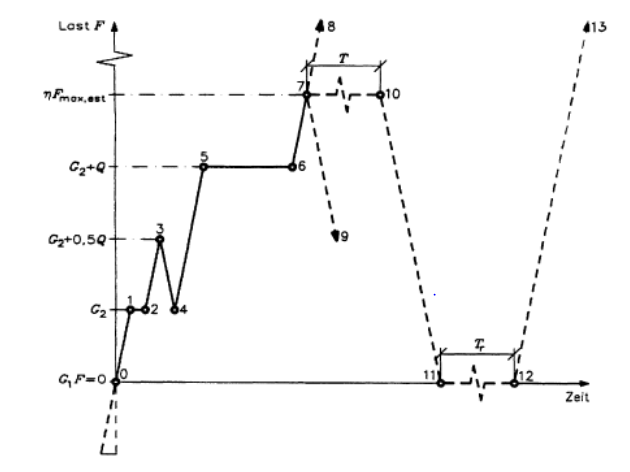
\includegraphics[width=12cm]{belastungskurve.png}
	\caption{Schematische Belasungskurve}
	\label{belastungskurve}

\end{center}	
\end{figure}	

\begin{table}
\caption{Grundlagen der Belastung}
\begin{center}
\begin{tabular}{|c|c|c|c|}
\hline 
Verfahrensstufe & Belastungsverfahren & Zeit in [s] & F [kN] \\ 
\hline \hline
0 & Es wirkt nur G;F=0 &  &  \\ 
\hline 
0-1 & F=G aufbringen &  & 2,70 \\ 
\hline 
1-2 & F=G konstant halten & 120 & 2,70 \\ 
\hline 
2-3 & F=G+0,5*Q aufbringen & 120 & 5,40 \\ 
\hline 
3-4 & 0,5 Q entlasten & 120 & 2,70 \\ 
\hline 
4-5 & F=G+Q aufbringen & 240 & 8,10 \\ 
\hline 
5-6 & F=G+Q konstant halten & 600 & 8,10 \\ 
\hline 
6-8 & F= steigern bis Bruch &  &  \\ 
\hline \hline
\multicolumn{4}{|c|}{ max. Belastungsgeschwindigkeit 0,25Q je 60 sec} \\ 
\hline 
\end{tabular} 
\label{tab:belastung}
\end{center}
\end{table}

















	
	
	
	
	
	
	
\chapter{Auswertung der Versuche}

\section{Allgemeines}

In diesem Kapitel werden die Unterschiede zwischen den 4 Versuchen erläutert und die Ergebnisse, sowie das Versagen der einzelnen Versuche erklärt. Weiters werden allgemeine Anmerkung zu dem Versuchen beschrieben. 

Die Tabelle \ref{tab:Versuchsprogramm}  soll einen Überblick über die Großbauteilversuche bzw. über die Unterschiede der einzelnen Versuche geben.
\begin{table}
\caption{Versuchsprogramm}
\begin{center}


\begin{tabular}{|c|c|c|c|c|c|}
\hline 
\multicolumn{6}{|c|}{ Versuchsübersicht} \\ 
\hline 
Versuch & Abmessungen  & Schraubenanzahl & Kleber & Belastung & Aushärtezeit \\ 

&  l x b x h in [m] & (Fa. SFS) & (FA. Sika) & (kN/mm$^{2}$] & Tage \\ 
\hline\hline
1 & 7,40 x 0,50 x 0,33 & 28 & Sikadur 31 & 4 & 14 \\ 
\hline 
2  & 7,40 x 0,50 x 0,33 & 8 & ElastoCem 109 & 4 & 21 \\ 
\hline 
3 & 7,40 x 0,50 x 0,33 & 12 & Sikatop 107 & Kapitel 3.7 & 28 \\ 
\hline 
4  & 7,40 x 0,50 x 0,33 & - & Sikatop 107 & Kapitel 3.7 & 28 \\ 
\hline 
\end{tabular} 
\end{center}
\label{tab:Versuchsprogramm}
\end{table}
\section{1 Versuch}

\subsection{Anmerkung:}

Der Schichtenaufbau ist wie im Kapitel 3 beschrieben. Die Anordnung der Schrauben ist aus der Abbildung \ref{1versuch} zu entnehmen. Es wurde wie in der Tabelle..  aufgelistet, der Kleber SikaDur 31-A Normal verwendet. 
Aufbau des Versuchskörpers mit Schraubenbild:


\begin{figure}[h]
\begin{center}
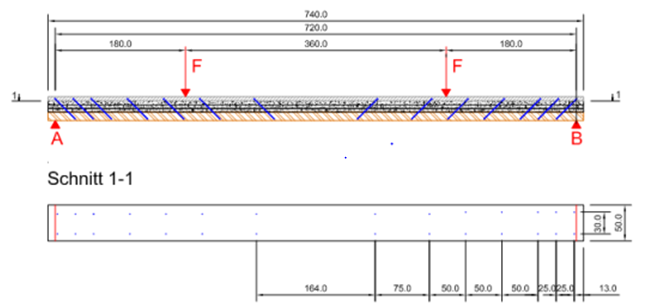
\includegraphics[scale =1.0]{1versuch.png}
\caption{Anordnung der Messpunkte}
\label{1versuch}
\end{center}
\end{figure}

\subsection{Versagensbeschreibung}


\begin{figure}[h]
\begin{minipage}[hbt]{7cm}
	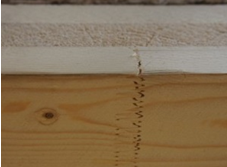
\includegraphics[width=6cm]{keilzinkung.png}
	\caption{Versagen der Keilzinkung }
	\label{keilzinkung}
\end{minipage}
\hfill
\begin{minipage}[hbt]{7cm}
Das erste Versagen wurde bei einer Last von 58 kN festgestellt. Unter der Last F vom Auflager B, brach eine Keilzinkung der Brettsperrholzplatte. In der Abbildung \ref{keilzinkung} ist der Schaden am Bauteil darstellt.
Beim weiteren Belasten traten zunächst Risse im Beton zwischen der Kraft F und dem Auflager B auf
\end{minipage}
\end{figure}


\begin{figure}[h]
\begin{minipage}[hbt]{7cm}
	\includegraphics[width=6cm]{bruch.png}
	\caption{Bruch nach Wiederbelastung }
	\label{bruch}
\end{minipage}
\hfill
\begin{minipage}[hbt]{7cm}
Schließlich hat bei 78 kN ist die Verbundfuge zwischen Holz und Holzspanbeton im Bereich zwischen dem Betonriss und dem Auflager B versagt. Dadurch entstand ein deutlicher Lastabfall und bei einer neuerlichen Belastung brach der Versuchskörper bei 48 kN vollständig ab.
\end{minipage}
\end{figure}

\begin{figure}
\begin{minipage}[hbt]{5cm}
	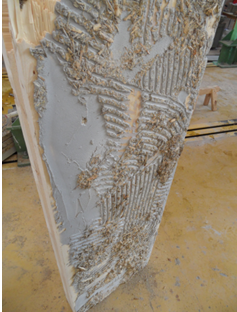
\includegraphics[width=6cm]{bruchbild.png}
	\caption{Bruchbild der CLT-Platte }
	\label{bruchbild}
\end{minipage}
\hfill
\begin{minipage}[hbt]{7cm}
Durch den Bruch konnte danach die Fuge zwischen Holzspanbeton und Holz betrachtet werden Abbildung \ref{bruchbild}. Es zeigte sich, dass ca. ein Viertel der Fläche ungenügenden Verbund hatte. Auf dieser Seite des Trägers brachen auch zwei Schrauben, die restlichen sechs Schrauben versagten durch Herausziehen aus der Brettsperrholzplatte.
\end{minipage}
\end{figure}

\clearpage


Der Hauptgrund für das Versagen der Verbundfuge und der Keilzinkung in Bereich zwischen Auflager A dürfte in der ungenügenden Vernetzung der Klebeschicht zwischen Holz und Holzspanbeton liegen. Durch den unzureichenden Verbund kam es zu höheren Biegespannungen in den Teilquerschnitten Holz und Beton und damit zum Bruch der Keilzinkung.
\newline
\subsection{Auswertung des 1 Versuchs}
 In dem Diagramm sind die Ergebnisse des  1 Versuchs dargestellt.




\begin{figure}
\begin{center}
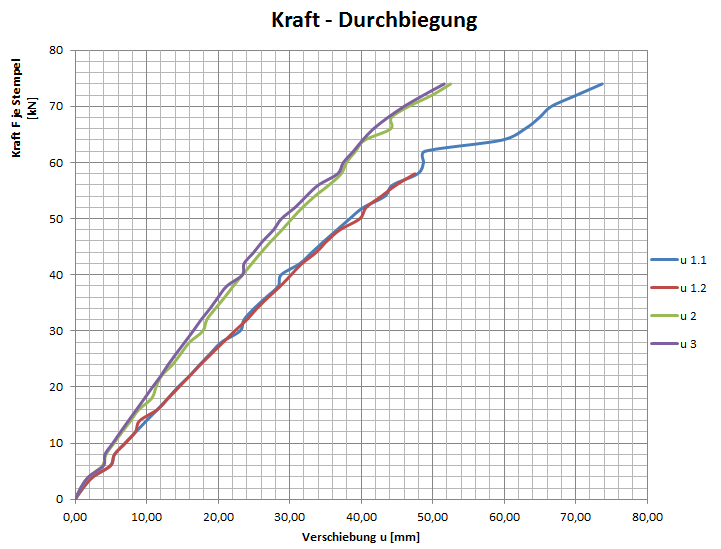
\includegraphics[scale =0.9]{1_versuch_kraft_durchbiegung.png}
\caption{1 Versuch: Kraft-Durchbiegung}
\label{1 Versuch: Kraft-Durchbiegung}
\end{center}
\end{figure}

Die Verschiebungen wurden nicht in Trägermitte gemessen, sondern am Rand der Träger, damit man die Verschiebung ablesen konnte, ohne im Gefahrenbereich des Trägers zu sein. Um eine eventuelle Torsion im Versuch ausschließen zu können wurde in der Trägermitte zwei Messuhren am Rand angebracht. Wie im Diagramm ersichtlich besteht kein Unterschied zwischen den Messpunten u 1.1 und u 1.2 . Die Differenz zwischen u 2 und u 3 ist minimal und kann auf Messfehler zurückgeführt werden. Ab dem Zeitpunkt der Kraft von 58 kN steigt die Differenz stark an, da ab diesem Zeitpunkt die Keilzinkung an der Stelle u 2 gerissen ist. 


\begin{figure}
\begin{center}
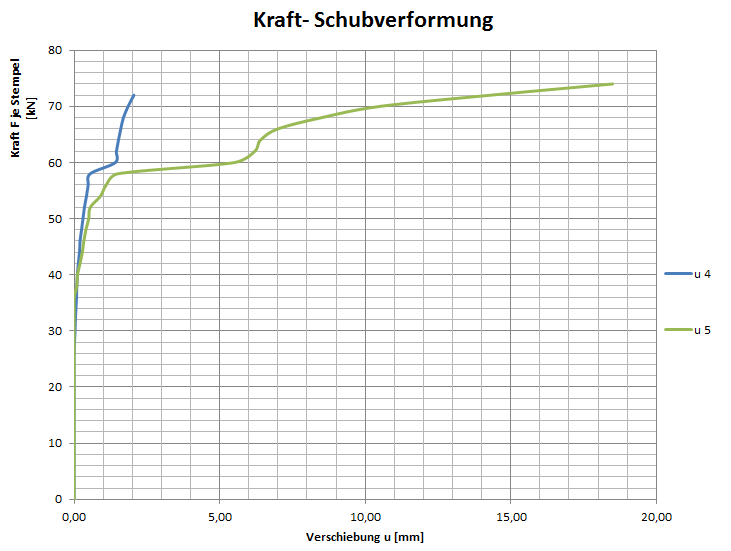
\includegraphics[scale =0.9]{1_versuch_kraft_schubverschiebung.png}
\caption{1 Versuch: Kraft-Schubverformung}
\label{1_versuch_kraft_schubverschiebung}
\end{center}
\end{figure}

Das Diagram stellt die relative Schubverformung zwischen der CLT-Schicht und der Betonschicht dar. Es ist auch in diesem Diagramm erkennbar, das bei 58 kN der Verbund der eizelenen Schichten nicht mehr vorhanden war. Der Auschlag der Kennlinie u 5 ist um ein vielfaches größer, da auf dieser Seite des Träger die Keilzinkung versagte und somit ein erheblicher Widerstandverlust auftrat.
\clearpage{}

\subsection{Schubversuch}


In einem ersten Schritt des Versuchskörpers wurde der gesamte Träger abgedrückt, mit dem 4-Punktbiegeversuch. Der Träger wurde nur auf einer Seite zerstört, auf der anderen Seite waren keine Beschädigungen ersichtlich. Somit wurde ein weiterer Verwendungszweck gesucht, um den nicht beschädigten Trägerteil zu nutzen. In der Abbildung \ref{träger_scherversuch}. ist ersichtlich welche Teile des Trägers verwendet wurden. 


\begin{figure}[h]
\begin{center}
\includegraphics[scale =0.9]{träger_scherversuch.png}
\caption{Darstellung des verwendeten Teiles der Trägers}
\label{träger_scherversuch}
\end{center}
\end{figure}

\paragraph{Erklärung des Schubversuchs}

\begin{figure}
\begin{minipage}[hbt]{8cm}
	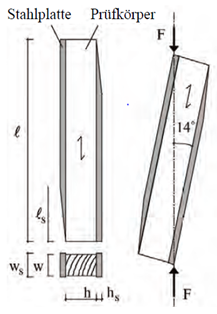
\includegraphics[width=5cm]{versuchsschema_scherversuch.png}
	\caption{Versuchsschema: Scherversuch }
	\label{versuchsschema_scherversuch}
\end{minipage}
\hfill
\begin{minipage}[hbt]{8cm}
Die Ermittlung von Scher- bzw. Schubfestigkeiten für den Holz und vor allem für  Sandwichbauteil existiert die Problematik, dass es nahezu unmöglich ist, einen reinen Schubspannungszustand zu erzeugen. Durch die geringe innere Festigkeit des Velox, sind die gängigen Prüfverfahren nicht anwendbar. 
Im Wesentlichen haben sich heute zwei Prüfverfahren zur Ermittlung der Schubfestigkeit von Holz etabliert, welche den einschlägigen Normen in verschiedenen Ländern zugrunde liegen. Im Europäischen Raum bezieht sich der [DIN EN 1995-1-1] auf die [DIN EN 408] wo das in Prüfverfahren erläutert wird. Dieser Versuchsaufbau wurde von uns adaptiert um das Verformungsverhalten der Verbundfuge zu untersuchen. Bei unserem Sandwichbauteil kommt anstatt der Stahlplatte, zum einem eine CLT-Platte und zum anderen eine SCC-Schicht zum Einsatz.

\end{minipage}
\end{figure}

\clearpage{}

Der Vorteil dieses Versuchsaufbaus liegt darin, dass der Bauteil in keiner Richtung gehalten werden muss und somit keine Querkräfte ableitet. Es wird die aufgebrachte Kraft durch die Verbundfuge des Bauteils abgeleitet.

\paragraph{Abemessungen und Versuchsdarstellung}





\begin{enumerate}
\item Versuch: 150 x 50 x 33,8 cm
\item Versuch: 100 x 50 x 33,8 cm
\end{enumerate}

\begin{figure}
\begin{minipage}[hbt]{7cm}	
	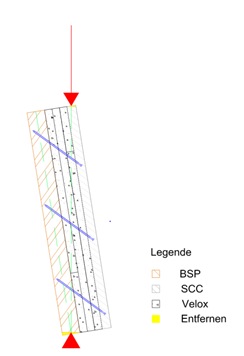
\includegraphics[width=8cm]{versuchsdarstellung_scherversuch_zeichnung.png}
	\caption{Zeichung der Scherversuchdarstellung}
	\label{Zeichung der Scherversuchdarstellung}
\end{minipage}
\hfill
\begin{minipage}[hbt]{7cm}
	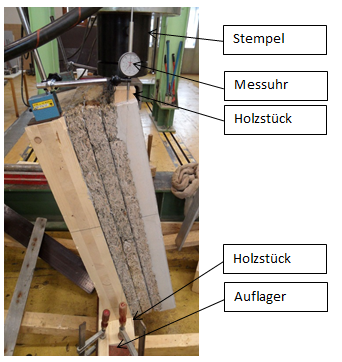
\includegraphics[width=8cm]{versuchsdarstellung_scherversuch_real.png}
	\caption{Darstellung des Scherversuchs}
	\label{Darstellung des Scherversuchs}
\end{minipage}
\end{figure}


\paragraph{Messeinrichtung}

\begin{figure}[h]
\begin{minipage}[hbt]{8cm}
	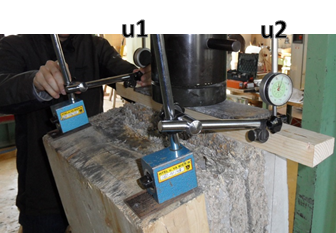
\includegraphics[width=5cm]{messeinrichtung_scherversuch.png}
	\caption{Anordnung und Darstellung der Messmittel }
	\label{messeinrichtung_scherversuch}
\end{minipage}
\hfill
\begin{minipage}[hbt]{8cm}
Es wurden für den Versuch 2 Messuhren am oberen Punkt des Bauteils mittels einer Stahlplatte angebracht. Somit konnte die Relativverschiebung zwischen der CLT- Schicht und der SCC-Schicht gemessen werden.

\end{minipage}
\end{figure}

\paragraph{Versuchsablauf}
 
Damit der Versuchsbauteil die schräge Lage einnimmt, wurde Holzstücke entsprechend der Neigungen angefertigt. Aufgrund der Unterschiedlichen Höhen der Versuchskörper waren diese Holzstücke unterschiedlich. Um ein verrutschen des Holzauflagers zu verhindern, wurden Befestigungszangen verwendet.
Zu Beginn des Versuchs wurde eine Referenzkraft von 0,5 kN aufgebracht. Die Messuhren wurden anschließend auf Null zurückgestellt.
Die Kraft wurde mit einer Geschwindigkeit von 1kN pro 10 Sekunden aufgebracht. Um die Verschiebung messen zu können sind Messuhren verwendet worden. Das Ablesen der Verschiebung erfolgte manuell von den Messuhren.

\begin{figure}
\begin{minipage}[hbt]{7cm}	
	\includegraphics[width=8cm]{bruchbild1_scherversuch.png}
	\caption{bruchbild scherversuch}
	\label{bruchbild scherversuch}
\end{minipage}
\hfill
\begin{minipage}[hbt]{7cm}
	\includegraphics[width=8cm]{bruchbild2_scherversuch.png}
	\caption{bruchbilder scherversuch}
	\label{bruchbilder scherversuch}
\end{minipage}
\end{figure}

Auf den Bruchbildern ist erkennbar, dass die innere Festigkeit des Velox versagt hat. Der Kleber ist nur gering in das Velox eingedrungen und hat somit  wenige Bestanteile gebunden. Es sind teilweise Stellen erkennbar, die keinen oder nur geringen Anteil des Velox haben. Dies ist auf Verarbeitungsmängel zurückzuführen.
Als letzter hat das Holz, durch das Ausziehen versagt. 


\paragraph{Auswertung des Schubversuchs}

\clearpage{}


\begin{table}
\caption{Maximalbelastung der Schubversuche}
\begin{center}

\begin{tabular}{|c|c|}
\hline 
Versuch & Bruchkraft  \\ 
\hline 
1 & 359 [kN] \\ 
\hline 
2 & 345 [kN] \\ 
\hline 
\end{tabular} 


\end{center}
\end{table}




\begin{figure}
\begin{center}
\includegraphics[scale =0.9]{Scherversuch_Kraft_Verschiebungslinie.png}
\caption{Scherversuch Kraft Verschiebungslinie}
\label{Scherversuch Kraft Verschiebungslinie}
\end{center}
\end{figure}


\textbf{Conclusio:}
Es ist ersichtlich das die beiden Versuche die fast gleiche Bruchlast aufweisen. Jedoch ist die Verschiebung beim 2 Versuch um die Hälfte geringer. Der Verlauf der Kennlinie ist auch nicht ident, daher müssten verschiedene Mechanismen bei den  Versuchen unterschiedlich aufgetreten sein. 
Der Hauptgrund für die unterschiedliche Kennlinie wird sein, die Vorbelastung durch den  4 Punktbiegeversuch. Auch wenn visuell keine Beeinträchtigung der Versuchskörper zu sehen war, hatte die Klebefuge bzw. die innere Festigkeit vom Velox, beim zweiten Versuch keinen Beitrag zur Lastabtragung. Somit musste die ganze Kraft über die Schrauben abgetragen werden.  Beim zweiten Versuch ist ein ausgeprägtes Plateau ersichtlich. Daher kann man davon ausgehen, dass vor dem Plateau die Schrauben und das Velox die Last abgetragen haben. Danach ist die Schraube alleine für die Lastabtragung verantwortlich. Die Steigung der Kennlinie bekräftigt die die oben beschriebene Vermutung, dass das System steifer ist als beim ersten Versuch. Beim zweiten Versuch ist die kein Plateau ersichtlich daher keine Beitrag vom Velox und somit eine geringe Steifigkeit des Systems.
Der Unterschied in den Verschiebung könnte durch die beschriebenen Steifigkeitsunterschiede abgeleitet werden. Die Schrauben werden beim 2 Versuch noch durch die intakte Verbundfuge 
unterstützt, daraus ergibt sich eine geringere Verschiebung in der ersten Phase des Versuchs.



\begin{figure}
\begin{center}
\includegraphics[scale =0.9]{Vergleich_Schubersuch.png}
\caption{Vergleich der Kennlinien nach 230 kN}
\label{VergleichSchubersuch}
\end{center}
\end{figure}

Vergleicht man die Kennlinien explizit nur in der Phase nach dem Plateau bzw. ab der Stelle wo nur noch die Schrauben zur Lastableitung beitragen, ist die Kennlinie nahezu ident. Das heißt der Unterschied zwischen den Versuchskennlinien, kann man auf die unterschiedliche Ausganglage (Vorschädigung) der Versuchskörper zurückführt werden. 


\section{2 Versuch}

\subsection{Anmerkung:}

Der Schichtenaufbau ist wie im Kapitel 4 beschrieben. Die Anordnung der Schrauben ist aus der Abbildung \ref{2versuch} zu entnehmen. Es wurde wie in der Tabelle..  aufgelistet, der Kleber ElastoCem 109  verwendet. 
Aufbau des Versuchskörpers mit Schraubenbild:


\begin{figure}
\begin{center}
\includegraphics[scale =0.8]{2versuch.png}
\caption{Darstellung des Versuchskörpers}
\label{2versuch}
\end{center}
\end{figure}

\clearpage{}
\subsection{Vorbemerkung}

Der Versuchskörper hat wie im Anschluss dargestellt, einige Schädigungen aufgewiesen. Es sind die Ergebnisse daher mit Vorsicht zu sehen. Auf den beiden Enden des Bauteil hatte sich die obersten Schichten der Veloxplatten von einander abgehoben. Weiters waren noch Risse in der Betonschicht im Bereich der $\frac{1}{4}$ Punkte zu sehen.
Die Schädigung sind beim Einlegen des Trägers in die Prüfanlage aufgetreten. Der Träger wurde mit 2 Gurten eher mittig angehoben und erfuhr daher einen Lastzustand der nicht vorgesehen war. Durch die mittige Anhebung war ein Kragarm and den Enden  mit ca. 2,50m Länge entstanden. Womit sich die Zug und Druckzone umgekehrt hat. So entstanden die Risse im Beton, zuerst in der Mitte des Träger und darauffolgend im Bereich der $\frac{1}{4}$ Punkte. Das Abheben der oberen Veloxschichten ist auf den verwendeten Kleber zurückzuführen. Er hatte zu geringe Klebeeigenschaften und es wurde laut einer Expertenaussage (Hr. Rössler)  der Kleber zu gering aufgetragen.
Es ist noch festzuhalten das beim 1 Bauteilversuch ident vorgegangen worden ist. Aufgrund der Verringerung der Schraubenanzahl und der Verwendung eines anderen Klebers, ist ein Bauteil entstanden, der eine geringe Steifigkeit hat. Dies ist der Grund für die Schädigung des Bautteils.

\begin{figure}
\begin{minipage}[hbt]{7cm}	
	\includegraphics[width=8cm]{schädigung_velox.jpg}
	\caption{schädigung velox}
	\label{schädigung velox}
\end{minipage}
\hfill
\begin{minipage}[hbt]{7cm}
	\includegraphics[width=8cm]{schädigung_scc.jpg}
	\caption{Schädigung des Betons}
	\label{schädigung scc}
\end{minipage}
\end{figure}



\subsection{Versagensbeschreibung}



\begin{figure}
\begin{center}
\includegraphics[scale =0.5]{2versuch_versagen.jpg}
\caption{Darstellung des Versagen}
\label{2versuch versagen}
\end{center}
\end{figure}



\begin{figure}
\begin{minipage}[hbt]{7cm}	
	\includegraphics[width=8cm]{2versuch_1oberfläche_velox.jpg}
	\caption{Oberfläche der aufgetragenen Schicht}
	\label{schädigung velox}
\end{minipage}
\hfill
\begin{minipage}[hbt]{7cm}
	\includegraphics[width=8cm]{2versuch_2oberfläche_velox.jpg}
	\caption{Oberfläche der aufgelegten Schicht}
	\label{schädigung scc}
\end{minipage}
\end{figure}

\subsection{Auswertung des 2 Versuchs}

\begin{figure}
\begin{center}
\includegraphics[scale =0.9]{2versuch_kraft_durchbiegung.png}
\caption{2 Versuch: Kraft-Durchbiegung}
\label{2 Versuch: Kraft-Durchbiegung}
\end{center}
\end{figure}

Die Verschiebungslinie im Messpunkt 1 ist in der Mitte des Trägers gemessen und legt bis zu 25 kN ein lineares Verhalten vor. Die Sprung bei 8 kN bzw bei 10 kN wird durch das Ablesen bedingt sein. Nach den 25 kN ist die Kennlinie deutlich flacher daher wird der gesamte Verbund von der Zwischenschicht (Velox) nicht mehr gegeben sein. Die weitere Laststufe wird durch die Schrauben aufgenommen. Eine weitere Laststeigerung war nicht mehr möglich, daher ist es schwierig zu sagen, ab welchen Zeitpunkt die Schrauben komplett ausgerissen sind.
Die Kennlinien der Messpunkte 2 und 3 sind bin zu 10 kN ident, danach sind schon unterschiede in der Verformung erkennbar. Die Unterschiede können wiederum auf die manuelle Auswertung geführt werden. Im Versuchsablauf waren  keine unsymmetrischen Schädigungen aufgetreten oder erkennbar. Bei der Last von 25 kN ist in der Kennlinie 3 (grün)  ein makanter Knick aufgetreten, d.h. der ist ein weitere Schädigung oder ein Versagen aufgetreten. 



\begin{figure}[h]
\begin{center}
\includegraphics[scale =0.9]{2versuch_kraft_schubverformung.png}
\caption{2 Versuch: Kraft-Schubverformung}
\label{2_versuch_kraft_schubverschiebung}
\end{center}
\end{figure}

Der Verschub zwischen den CLT-Schicht und der Betonschicht ist in den Kennlinien 4 und 5 abgebildet. Die Kennlinie sind nahezu ident und weisen bis zu 25 kN ein liniares verhalten auf. Danach ist ein leicht progressiver Anstieg erkennbar.

Die Kennlinien sind bis zu der Laststufe von 25 kN linear aufgetreten, dies ist in jedem Messpunkt ersichtlich. Ab dieser Laststufe sind größere Verschiebungen ersichtlich. Es wird hier die Beginn des Auszug der Schrauben sein


\section{3 Versuch}

\subsection{Anmerkung:}
Der Schichtenaufbau ist wie im Kapitel 3 beschrieben. Die Anordnung der Schrauben ist aus der Abbildung …. zu entnehmen. Es wurde wie in der Tabelle..  aufgelistet, der Kleber Sikatop 107 verwendet. 

\begin{figure}
\begin{center}
\includegraphics[scale =0.8]{3versuch.png}
\caption{Darstellung des Versuchskörpers}
\label{3versuch}
\end{center}
\end{figure}

\clearpage{}



\section{4 Versuch}

\subsection{Anmerkung:}
Der Schichtenaufbau ist wie im Kapitel 3 beschrieben. Die Anordnung der Schrauben ist aus der Abbildung …. zu entnehmen. Es wurde wie in der Tabelle..  aufgelistet, der Kleber Sikatop 107 verwendet. 

\begin{figure}[h]
\begin{center}
\includegraphics[scale =0.8]{4versuch.png}
\caption{Darstellung des Versuchskörpers}
\label{4versuch}
\end{center}
\end{figure}

\clearpage{}

\chapter{Berechnungen}

\section{$\gamma$ - Verfahren}

Das Gamma- Verfahren wird zur Berechnung von Bauteilen verwendet, die einen nachgiebigen Verbund aufweisen. In der Abbildung…. sind die verschiedenen Verbundarten dargestellt.
Bei dem Sandwichaufbau Holz-Holzbeton werden verschiedene Baustoffe verwendet und  nachträglich miteinander verbunden. Zum Einsatz als Verbindungsmittel kommen: Kleber und Schrauben. Daher spielt die Anordnung und Verwendung der  Verbindungsmittel eine entscheidende Rolle über die Aussage des Verbundes.  Dies muss bei der statischen Berechnung berücksichtigt werden. 


Abhängig vom Verbund ergeben sich unterschiedliche Spannungsverteilungen, wie in der Abbildung…….. dargestellt.

\begin{figure}
\begin{center}
\includegraphics[scale = 0.5]{verbunddarstellung.jpg}
\caption{Auswirkungen des nachgiebigen Verbundes auf die Spannungsverteilungen}
\label{verbunddastellung}
\end{center}
\end{figure}

Wie aus Abb…….. hervorgeht, ist das Ebenbleiben des Gesamtquerschnittes nach der Bernoulli-Hypothese nicht mehr gewährleistet. Somit können die Regeln der Technischen Biegelehre nicht auf nachgiebig miteinander verbundene Systeme angewendet werden. In der DIN 1052 [] sind zwei unterschiedliche Verfahren aufgeführt, die für die Schnittgrößenermittlung derartiger Systeme angewendet werden können:

\begin{itemize}
\item $\gamma$ -Verfahren Abs. 8.6.2 der DIN 1052 []
\item Schubanalogie Anhang D der DIN 1052 []
\end{itemize}



Im Teilbericht 15 der TU München [] sind die Anwendungsgrenzen für das  $\gamma$ -Verfahren angeführt.:
\begin{itemize}

\item statisch bestimmter Einfeldträger
\item sinusförmige Belastung
\item konstante Querschnitte (max. drei Teilquerschnitte)
\item Gültigkeit der Bernoulli-Hypothese in den Teilquerschnitten
\item kontinuierlicher, konstanter Verbund
\item Vernachlässigung der Schubverformung der Teilquerschnitte
\end{itemize}

Für den baupraktisch relevanten Fall der Gleichlast bildet das $\gamma$ -Verfahren eine gute Näherung. Auch Schnitt- und Verformungsgrößen an Durchlaufträgern ermittelt werden.
Generell berücksichtigt das $\gamma$ -Verfahren die Abnahme der Biegesteifigkeit des Verbundquerschnitts aufgrund der Nachgiebigkeit der Verbundfuge durch den Abminderungsfaktor $\gamma$. 
Dieser reduziert nur die Steineranteile der Biegesteifigkeiten der Teilquerschnitte während die Eigenanteile unverändert bleiben.
In der Anwendung für den Bauteil Holz-Holzspanbeton ist das Verfahren nicht wie in der Literatur dargestellten Form anzuwenden. Durch die Anwendung des Holzspanbetons als Mittelschicht und dessen geringe Festigkeiten muss hier eine Abwandlung angewendet werden. Die Abwandlung wurde mit abgesprochen.
Der Bauteil wird so behandelt, wie wenn er nur aus zwei Bestandteilen bestünden würde und die Mittelschicht als duktile Klebeschicht. Daher verändert sich der Formelapparat.
Die Beiwerte der Querschnittsteile (i=1 und i=3), die nachgiebig an den Teilquerschnitt i=2 angeschlossenen sind, werden berechnet zu: 


\clearpage{}





\section{FEM-Sofistik}

\section{Vergleich Berechnungen}




\end{document}



